%\chapter{det-comp}


%%%%%%%%%%%%%%%%%%%%%%%%%%%%%%%%%%%%%%%%%%%%%%
%\section{Anode Plane Assemblies}

%%%%%%%%%%%%%%%%%%%%%%%%%%%%%%%%%%%%%%%%%%%%%%
%\section{Cathode Plane Assemblies}

%%%%%%%%%%%%%%%%%%%%%%%%%%%%%%%%%%%%%%%%%%%%%%
%\section{Field Cage}

%%%%%%%%%%%%%%%%%%%%%%%%%%%%%%%%%%%%%%%%%%%%%%
%\section{HV components}

%%%%%%%%%%%%%%%%%%%%%%%%%%%%%%%%%%%%%%%%%%%%%%
\section{TPC Front-end Electronics}
%\chapter{Cold Electronics}
\label{ch:ce}

%
%%%%%%%%%%%%%%%%%%%%%%%%%%%%%%%%
%\subsection{Introduction}
\subsection{Overview and requirements}
\label{subsec:ce_intro}

\begin{cdrfigure}[The front-end electronics mounted on an APA]{tpcce_FEMBonAPA}{The 
front-end electronics as mounted on an APA.
  {\bf Top:} The front-end electronics is shown in the red circle.
  {\bf Bottom:} Cross section view. Mounting hardware between the front-end electronics 
and the APA fin is not shown.}
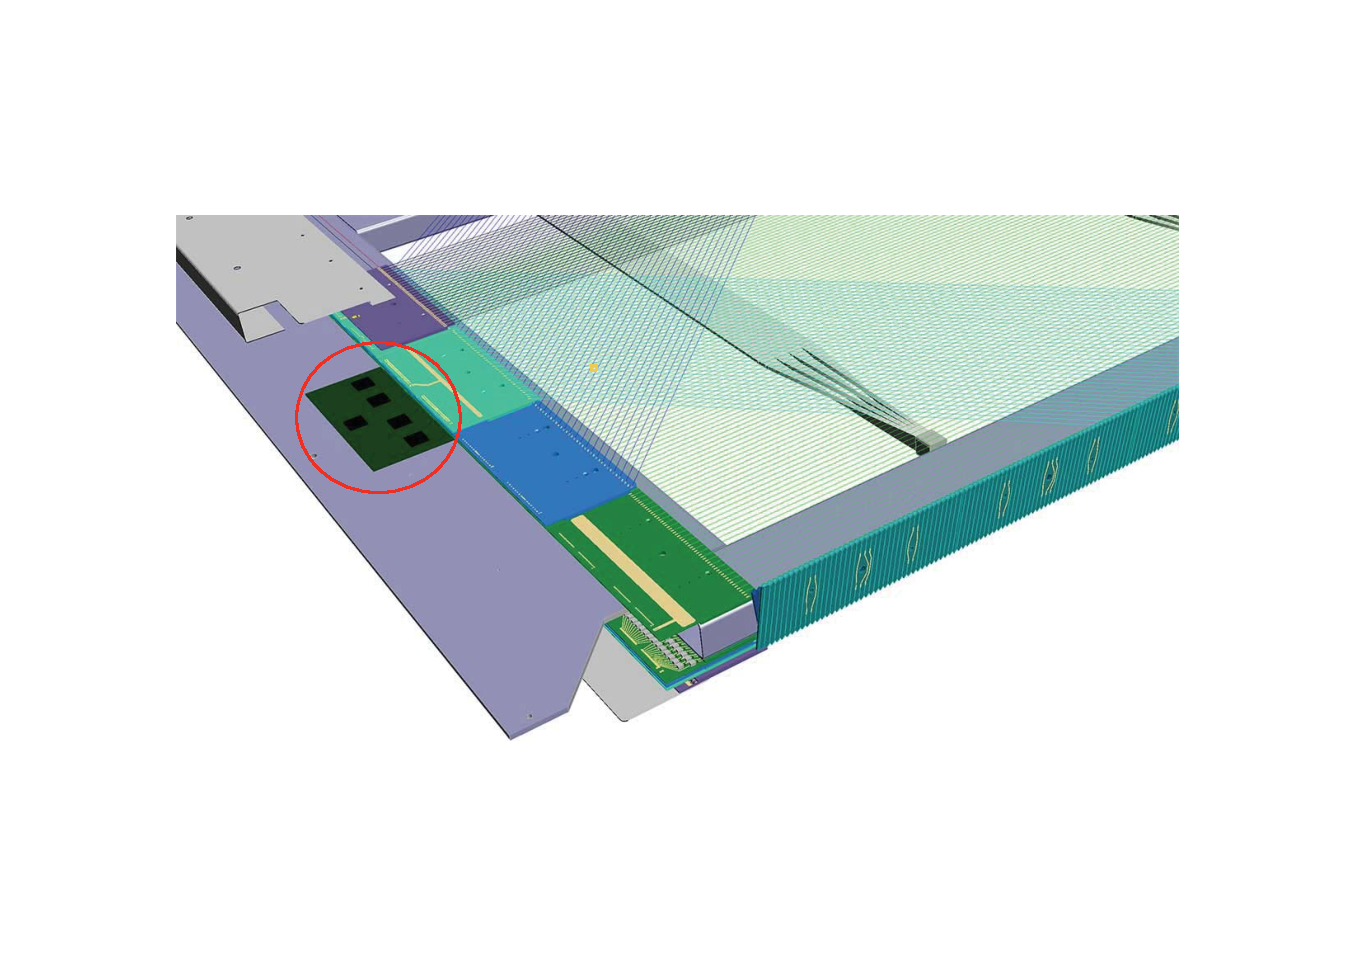
\includegraphics[width=0.8\linewidth]{tpcce_CMBonAPA_1.pdf}
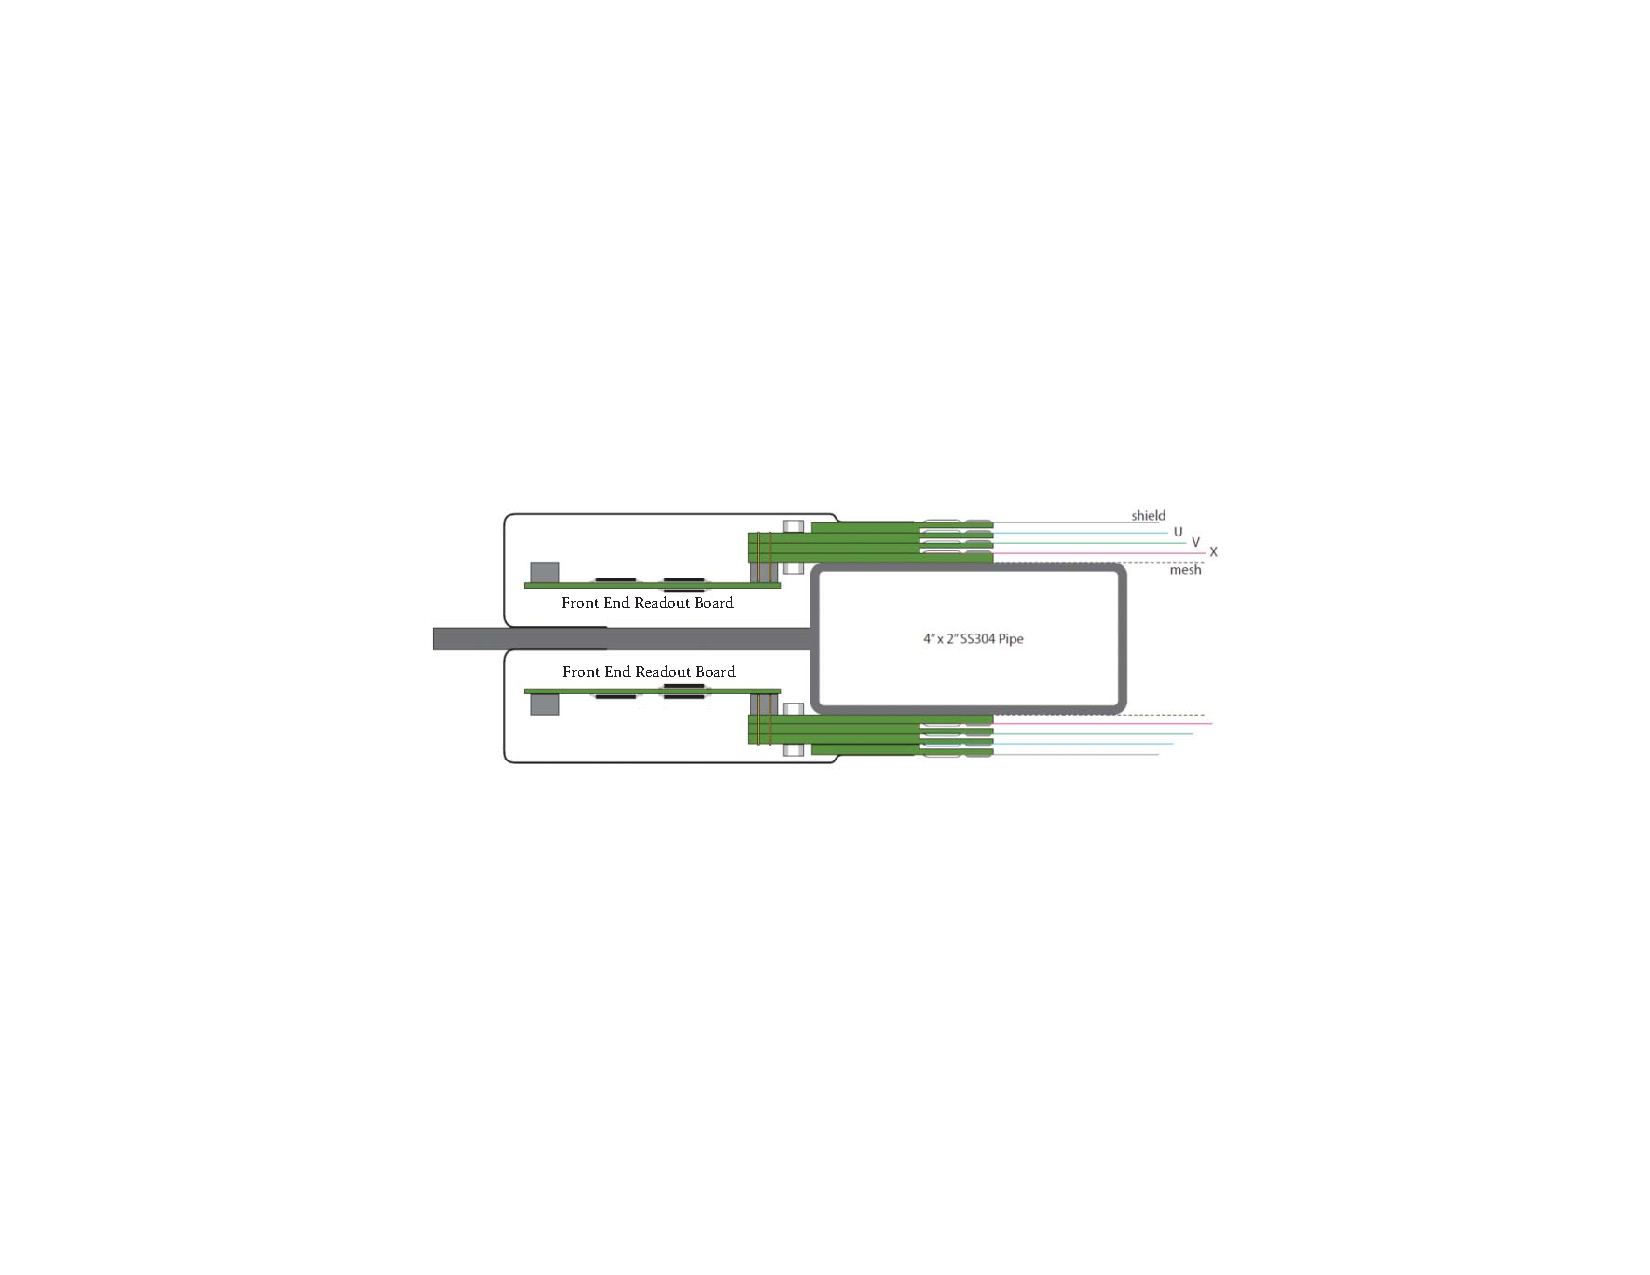
\includegraphics[width=0.8\linewidth]{tpcce_CMBonAPA_2.pdf}
\end{cdrfigure}

The DUNE single-phase TPC read-out electronics are referred to as the ``Cold Electronics'' (CE) because they will reside in LAr,
mounted directly on the APA front-end (Figure~\ref{fig:tpcce_FEMBonAPA}).
This will minimize channel capacitance and noise by keeping the length of the connection between an anode wire
and its corresponding electronics input to an absolute minimum.
The CE will be implemented as ASIC chips using CMOS technology,
which performs well at cryogenic temperatures,
and will provide amplification, shaping, digitization, buffering, and multiplexing (Mux) of the signals.
Because it is not possible to form a trigger for some important measurements,
such as proton decay and supernova bursts, the CE will be continuously read out,
with a digitized ADC sample from each APA channel (wire) up to every 500~ns (2~MHz maximum sampling rate).

In ProtoDUNE-SP, the 2,560 channels from each APA are read out by 20 Front-End Motherboards (FEMBs), each providing 
digitized wire read-out of 128 channels. A single front-end board is shown in Figure~\ref{fig:tpcce_FEMBonAPA}.
For each of the six APAs in the protoDUNE cryostat, one cable bundle will 
connect from each FEMB to the outside of the cryostat via a feedthrough to a CE flange, with one 
feedthrough/flange servicing one APA as shown in Figure~\ref{fig:tpcce_apa_flange},
for a total of 20 cold cable bundles per APA. 
Each of these cable bundles consists of wires for low-voltage power, links for high-speed data out,
and clock/digital-control IOs.
Eight other cables carry the TPC wire-bias voltage from the CE flange to the APA wire-bias boards, as
shown in Figure~\ref{fig:tpcce_cr_board}.

\begin{cdrfigure}[Connections between CE flange and APA]{tpcce_apa_flange}{Connections between
the CE flange and APA.}
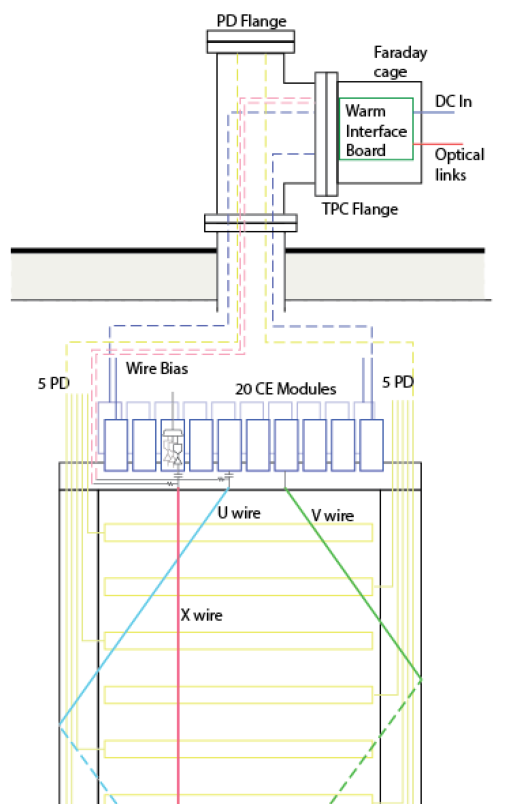
\includegraphics[width=0.4\linewidth]{tpcce_apa_flange.pdf}
\end{cdrfigure}

The scope of the CE subsystem includes the design, procurement, fabrication, testing,
delivery, and installation of the CE, the components of which are:
\begin{itemize}
\item Front-end mother boards (FEMBs) which include the cold ASICs, installed on the APAs
\item Data, clock/control IO, and LV and wire-bias power cables 
between the APA and the CE flanges (cold cable)
\item Signal feedthroughs and CE flanges which pass the data, clock/control IO, 
low-voltage power, and APA wire-bias voltage between warm and cold
\item Warm electronics crates (WECs) mounted on the CE flanges, which act as Faraday cages with
only optical fibers to slow control and the DAQ, and which contain the Warm Interface Boards (WIBs)
and Power and Timing Cards (PTCs)
\item Data and clock/control IO fiber cable between the WEC and the data acquisition 
(DAQ) and slow control systems
\item LV and wire-bias power cables between the CE flange and external power supplies (warm cable)
\item Low-voltage supplies for the CE and bias-voltage supplies for the APAs
\end{itemize}

%The responsibility and authority for the design, installation 
%and use of the detector quiet-power distribution and 
%detector-grounding system is held by the subproject electrical engineer. 
%This engineer has oversight responsibility for all electrical and electronics 
%design and installation tasks, including all attachments to the detector 
%that create an electrical connection. 

By ensuring that the electrical cables for each APA enter the cryostat through single 
independent feedthrough penetrations, the TPC APA, cold electronics read-out, CE flange, 
and Faraday cage Warm Electronics Crate for each independent APA are an integrated whole
read-out unit. Each unit will provide local diagnostics for noise and validation testing,
and follow the grounding guidelines in Section~\ref{subsec:ele_design}.

%
%%%%%%%%%%%%%%%%%%%%%%%%%%%%%%%%
%\subsection{Design Considerations} 
%\label{subsec:ce_reqs_n_specs}

The most significant requirements for the CE are listed here. The CE shall:

\begin{itemize}	
\item Provide the means to read out the TPC wires and transmit their data in a useful format to the DAQ.
\item Operate for the life of the facility without significant loss of function.
\item Record the channel waveforms continuously without dead time.
\item Use only materials that are compatible with high-purity liquid argon.
\item Provide sufficient precision and range in the digitization to:
\begin{itemize}
\item Discriminate electrons from photon conversions;
\item Optimize for high- and low-energy tracks from accelerator-neutrino interactions;
\item Distinguish a Minimum Ionizing Particle (MIP) from noise with a signal-to-noise ratio $>$ 9:1;
\item Measure the ionization up to 15 times that of a MIP particle, so that stopping kaons from proton decay can be identified.
\end{itemize}
\item Ensure that all power supplies have: 
\begin{itemize}
\item Local monitoring and control
\item Remote monitoring and control through DAQ
\item Over-current and over-voltage protection circuits
\end{itemize}
\item Ensure that the signal feedthroughs are able to withstand twice their nominal operating voltages 
with a maximum specified leakage current in 1-atm argon gas.
\end{itemize}


%%%%%%%%%%%%%%%%%%%%%%%%%%%%%%%%
%\subsubsection{Electrical design guidelines}
\subsubsection{Electrical design}
\label{subsec:ele_design}

To avoid structural ground loops, the APA frames described in Section~\ref{subsec:apa_frame} 
are insulated from each other. Each frame is electrically connected to the cryostat at a single 
point, where cold cables exit the cryostat signal feedthrough. Mechanical suspension of the APAs 
is accomplished using insulated supports. 

The FEMB \fixme{write out} include an analog motherboard with eight Front-End (FE) ASICS configured as 16-channel 
digitizing charge amplifiers. Input amplifiers on the ASICs have their Common terminals connected 
to the APA frame. These connections are made through the CE Faraday box described in 
Section~\ref{subsubsec:ce_faraday_box} and its mounting brackets. All power-return leads and all cable shields 
involving the CE are connected to the Common plane of the FEMB, as well as to the CE flange.

Bias filters are locally referenced to the Common plane of the FEMBs through low-impedance 
electrical connections. This approach keeps the ground-return path in close proximity to the 
bias-voltage and signal paths. Close proximity for the current paths minimizes loop areas to 
suppress noise pickup.

Photon Detector signals, described in Section~\ref{sec:pd_system}, are carried on shielded 
twisted pairs to a photon detector flange in the cryostat. The shields are connected to the 
cryostat at the PD flange, and to the PCB shield layer on the photon detectors. There is no 
electrical connection between the cable shields and the APA frame except at the PD flange.

%
%%%%%%%%%%%%%%%%%%%%%%%%%%%%%%%%
\subsection{APA wire bias}
\label{subsec:ce_wire_bias}

Each side of an APA includes four wire layers as described in Section~\ref{subsec:apa_phys_desc}. 
The inner-most X-plane layer of wires is nominally biased at +820 Volts, with each wire coupled 
to a charge amplifier in an FEMB. The V-plane layer of wires is effectively biased at zero volts, 
with each wire directly connected to a FE charge amplifier. The U-plane wire layer is nominally 
biased at -370 Volts with each wire coupled to a FE charge amplifier. The outer-most G-plane layer,
which is not connected to the FE charge amplifiers, is biased at -665 Volts.

Electrons passing through the wire grid must drift unimpeded until they reach the X-plane 
collection layer. The nominal bias voltages are predicted to result in an electrically 
transparent structure.

%%%%%%%%%%%%%%%%%
\subsubsection{Bias Components}
\label{subsec:ce_bias_comp}

For the wire layers, bias resistors and filter capacitors are mounted on CR boards that plug 
into the APA wire-board stacks, as described in Section~\ref{subsubsec:apa_wire_wrap}. The CR boards 
also plug directly into the FEMBs and make the electrical input to the FE amplifiers.

Each CR board includes two R-C filters for the X and U bias voltages, as shown 
in Figure~\ref{fig:tpcce_cr_board}. Additionally there are 48 
pairs of bias resistors and coupling capacitors for X-plane wires, and 40 resistor and 
capacitor pairs for the U-plane wires. The coupling capacitors block DC while passing AC 
signals to the CE motherboards.

\begin{cdrfigure}[APA wire bias schematic diagram]{tpcce_cr_board}{APA wire bias 
schematic diagram, including the Capacitance-Resistance (CR) board.}
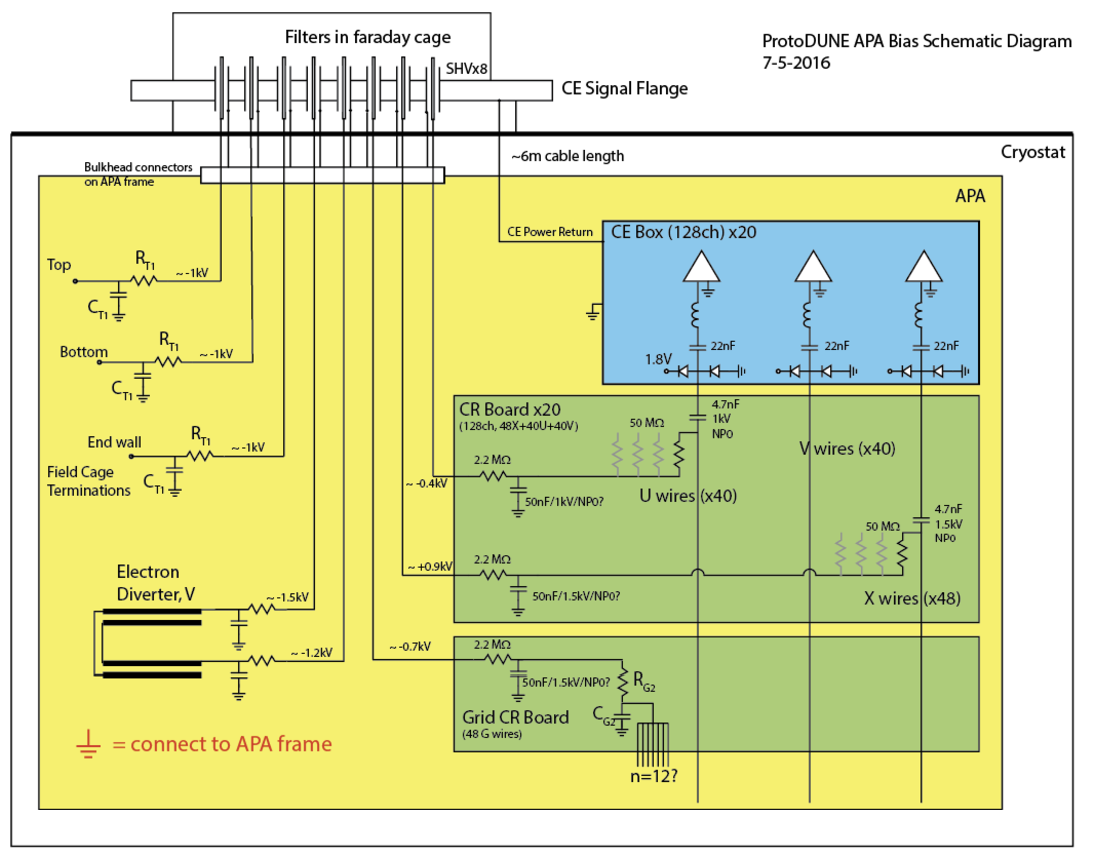
\includegraphics[width=0.8\linewidth]{tpcce_cr_board.pdf}
\end{cdrfigure}

A separate grid-plane CR board includes a bias voltage noise filter and twelve pairs of 
bias resistors and filter capacitors. Groups of four wires are tied together to share a 
bias resistor and filter capacitor. These CR boards do not provide input to the cold
electronics FE amplifiers.

The input amplifiers are referenced to the Common plane of the FEMB, which is locally connected 
to the APA frame through the CE Faraday box described in Section~\ref{subsubsec:ce_faraday_box}. The amplifiers 
have input impedance of 50 Ohms with 22-nF coupling capacitors, as shown in Figure~\ref{fig:tpcce_cr_board}. 
Clamping diodes limit the amplifier input voltage to between zero and +1.8 Volts.

%%%%%%%%%%%%%%%%%
\subsubsection{Bias Component Values}
\label{subsec:bias_comp_values}

Coupling capacitors for the X-plane and U-plane wires are required to block DC bias voltages.
However they also impact the efficiency of the detector circuits.
The sense wires are expected to have 200 pF of capacitance to the APA frame.
Induced or collected charges are effectively divided between the wire capacitance and the coupling capacitor.
To achieve a charge-calibration accuracy of 0.5 percent or better,
the coupling capacitors must be 4.7 nF at ten percent tolerance, or 2.2 nF at five percent tolerance.
Voltage ratings should be at least 1.5 times the expected operating voltages.

Bias resistance values should be at least 20 Meg-ohms to maintain negligible noise contributions.
A target value of 50 Meg-ohms is desired.
The higher value helps to achieve a longer time constant for the high-pass coupling networks.
Time constants should be at least 25 times the electron drift time so that the undershoot in the digitized waveform
is small and easily correctable.
However, leakage currents can develop on PC boards that are exposed to high voltages over extended periods.
If the bias resistors are much greater than 50 Meg-ohms, leakage currents may affect the bias voltages applied to the wires.

The bias-voltage filters are R-C low-pass networks.
Resistance values should be much smaller than the bias resistances to control crosstalk between wires
and limit the voltage drop if any of the wires becomes shorted to the APA frame.
A value around 2.2 Meg-ohms is desired.
Smaller values may be considered although a larger filter capacitor would be required to maintain a given level of noise reduction.
A target value of 47 nF has been established for the filter capacitors.

For the grid-plane bias filters, component values are less critical.
If possible they will be identical to those used for the bias resistors and coupling capacitors
(50 Meg-ohms and 2.2 to 4.7 nF).

Voltage ratings for the bias resistors and coupling capacitors, as well as their resistance and capacitance values,
are limited by available space on the CR boards.
The board area is limited by the width of the wire boards and the distance between the APA frame and the CE Faraday box.
Initial layouts have determined that the maximum possible size for the 88 bias resistors that must fit on each CR board
is 0.12 x 0.25 inches (3.0 x 6.0 mm).
Fortunately, resistors with this footprint are readily available with a voltage rating of 2.0 kV.
The maximum size for the 88 coupling capacitors on each CR board is 0.22 x 0.25 inches (5.6 x 6.0 mm).
Capacitors with a voltage rating of 2.0 kV are available with capacitance of 3.9 nF at five percent tolerance.

%
%%%%%%%%%%%%%%%%%%%%%%%%%%%%%%%%
\subsection{Front-End Mother Board}
\label{subsec:fe_arch}

The CE architecture is manifested in the FEMB assembly,
which consists of an analog mother board with a digital ASIC mezzanine (Figure~\ref{fig:tpcce_schem}).
Each APA is instrumented with 20 FEMBs, for a total of 2,560 channels per APA.
The FEMBs plug directly into the APA CR boards, making the connection from the U and V induction wires and 
Z collection wires to the FE charge amplifiers as short as possible.

The analog mother board is instrumented as a 128-channel board which uses eight 16-channel FE ASICs,
eight 16-channel ADC ASICs, low-voltage regulators, and input-signal protection.
The 16-channel FE ASIC provides amplification and pulse shaping.
The 16-channel ADC ASIC comprises a 12-bit digitizer at up to 2 MS/s, local buffering,
and an 8(analog):1(digital) Mux stage with two pairs of serial readout lines in parallel.
The FEMB has already been prototyped and tested,
using a commercial FPGA to perform the role of the digital ASIC (Figure~\ref{fig:tpcce_CMBpix}).

\begin{cdrfigure}[The CE Architecture]{tpcce_schem}{The CE Architecture. The basic unit is the 128-channel FEMB.}
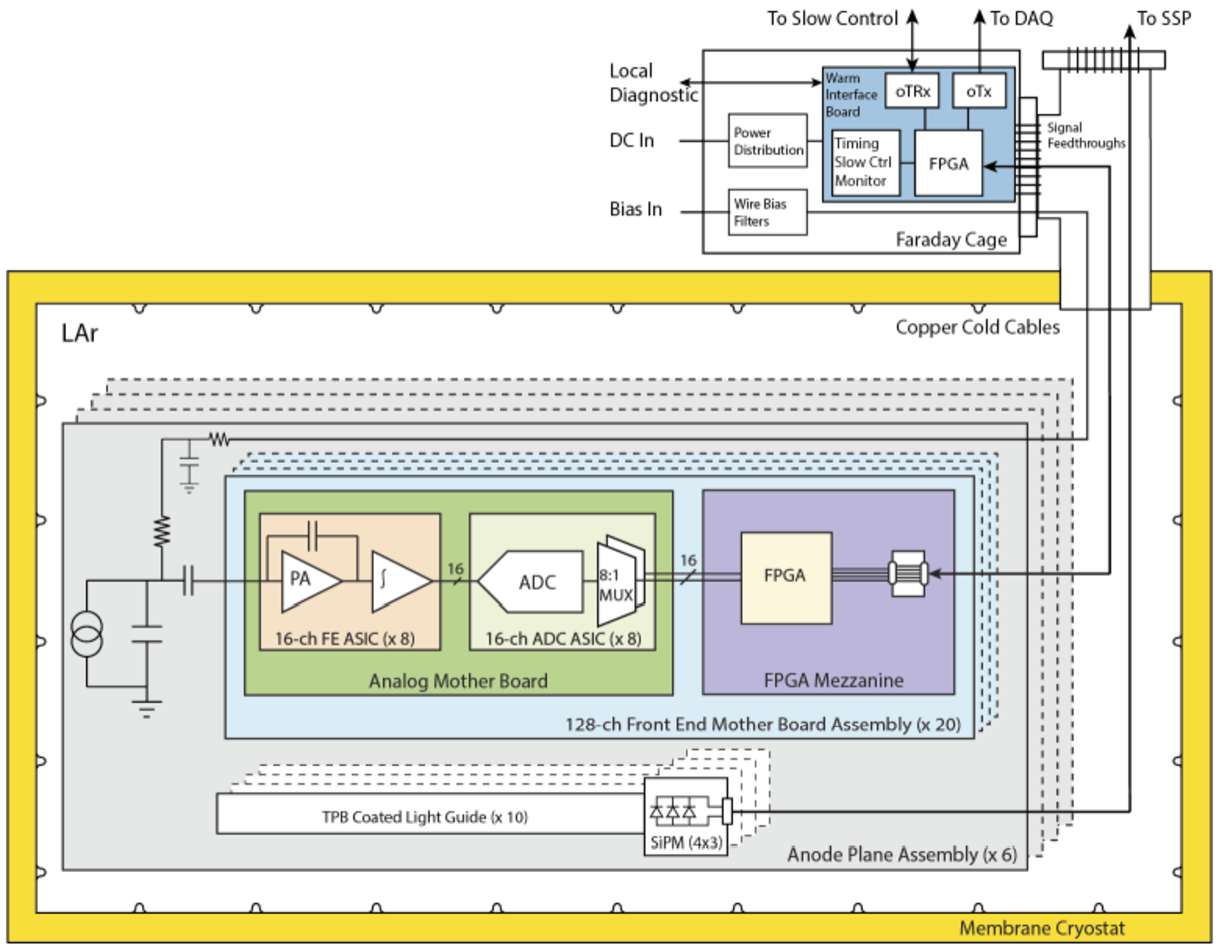
\includegraphics[width=0.9\linewidth]{tpcce_schem.pdf}
\end{cdrfigure}

\begin{cdrfigure}[The Front End Mother Board (FEMB), as used in an early set of tests]{tpcce_CMBpix}
{The Front End Mother Board (FEMB), as used in the early set of tests.
  {\bf Top:} The analog mother board, showing four ADC ASICs and four FE ASICs surface mounted.
  The other side of the board has another four ADC and FE ASICs.
  Except for anticipated small modifications, this board is essentially the final version.
  {\bf Middle:} The FPGA mezzanine, used in place of the digital ASIC mezzanine for the early set of tests.
  {\bf Bottom:} The complete FEMB assembly as used in the early set of tests.
  The cable shown in the high-speed data, clock, and control cable.}
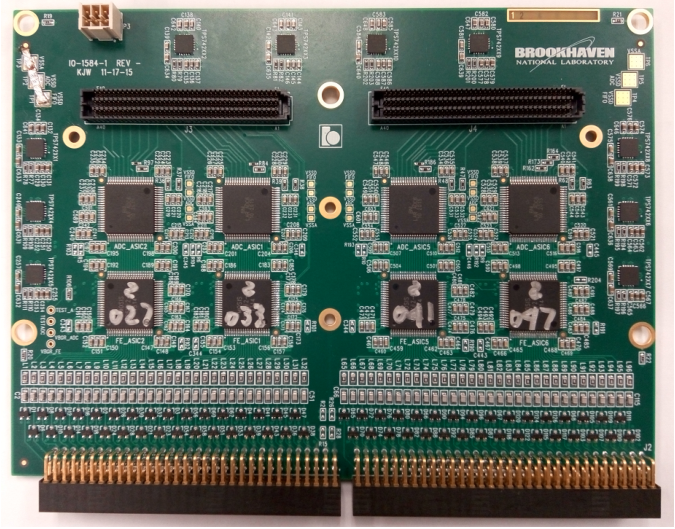
\includegraphics[width=0.65\linewidth]{tpcce_CMBpix_1.pdf}
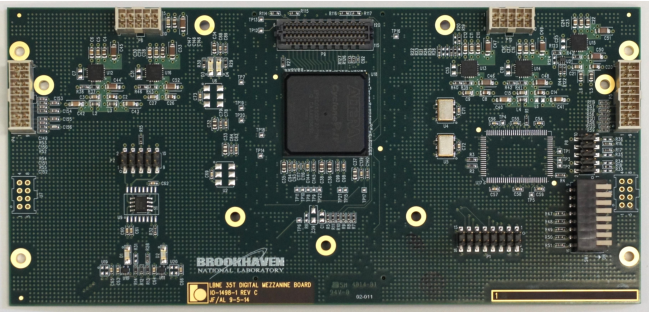
\includegraphics[width=0.65\linewidth]{tpcce_CMBpix_2.pdf}
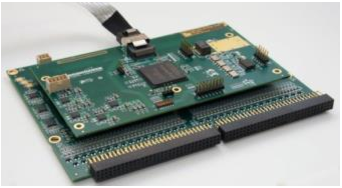
\includegraphics[width=0.45\linewidth]{tpcce_CMBpix_3.pdf}
\end{cdrfigure}

For a DUNE single-phase detector module, the Cold Digital Data (COLDATA) ASIC and its voltage regulators are mounted on the digital ASIC mezzanine.
The COLDATA ASIC will provide:
\begin{itemize}
\item The communication protocol with the DAQ
\item The control required to program and read out the FE and ADC ASICs
\item The system clock interface
\item Four 4:1 Muxs that combine 16 serial lines from the ADCs of eight 
channels each into four serial lines of 32 channels each
\item Four $\sim$1.2 Gigabit-per-second (Gbps) serial drivers that form the data link to the DAQ via the WIB
\end{itemize}
For the ProtoDUNE detector the COLDATA ASIC, which is still in development, will be 
emulated by an FPGA which will reproduce the clock/control IO, data multiplexing,
and $\sim$1.2~Gbps serial drivers.
The data rate will not be high enough to require the use of optical fibers in the cold,
nor is there a need for zero suppression or data compression.
%
Data will be driven to the CE flange through copper cable utilizing low-voltage differential signaling (LVDS).
At the CE flange, the data will be further multiplexed by 4:1 and transmitted over optical
fiber to the DAQ (RCE or FELIX) described in section~\ref{sec:DAQ_online_interface}.

The analog FE ASIC has 16 channels.
Each channel includes a charge amplifier with a gain selectable from one of 4.7, 7.8, 14 and 25~mV/fC
(full scale charge of 55, 100, 180 and 300~fC),
a high-order anti-aliasing filter with adjustable time
constant (peaking time 0.5, 1, 2, and 3 $\mathrm{\mu}$s),
an option to enable AC coupling,
and a baseline adjustment for operation with either the collecting (200~mV) or the non-collecting (900~mV) wires.
The 16-channel FE ASICs then transmit the shaped pulse to a 16-channel 12-bit 2~MS/s ADC ASIC.
Shared among the 16 channels in the FE ASIC are the bias circuits, programming registers,
a temperature monitor, an analog buffer for signal monitoring, and the digital interface.
The estimated power dissipation of FE ASIC is about 6~mW per channel at 1.8~V supply.
Shared among the 16 channels in the ADC ASIC are the bias circuits, programming registers,
an 8:1 Mux, and the digital interface.
The estimated power dissipation of FE ASIC is below 5~mW per channel at 1.8~V supply.


%
%%%%%%%%%%%%%%%%
\subsubsection{Cold Analog ASICs}
\label{subsubsec:fe_CMOS_analog}

The development of the readout ASIC began by designing and fabricating in a commercial CMOS
process (0.18~$\mu$m and 1.8V) a 16-channel ASIC implementing the complete analog front-end section.
The FE ASIC layout is shown in Figure~\ref{fig:tpcce_FE_ASIC}.
This process is expected to be available for at least another 10~years. 
The charge amplifier input MOSFET is a p-channel biased at 2~mA with a L/W (channel length/width) ratio
of 0.27~$\mu$m / 10~$\mu$m, followed by dual cascade stages.
The charge amplification and shaping filter have digitally programmable gain and peaking time
(as listed in Section~\ref{subsec:fe_arch}).
Each channel also implements a high-performance output driver,
which is used to drive a long cable when it is used in a standalone mode, as it is in MicroBooNE.\cite{noise_filter}
The buffer can be disabled when it is interfaced to an ADC ASIC to reduce the power consumption.
The ASIC integrates a band-gap reference (BGR) to generate all the internal bias voltages and currents.
This guarantees a high stability of the operating point over a wide range of
temperatures, including cryogenic.
The ASIC is packaged in a commercial, fully encapsulated plastic QFP 80 package.

\begin{cdrfigure}[The layout of the 16-channel analog FE ASIC]{tpcce_FE_ASIC}{The layout of the 16-channel analog FE ASIC}
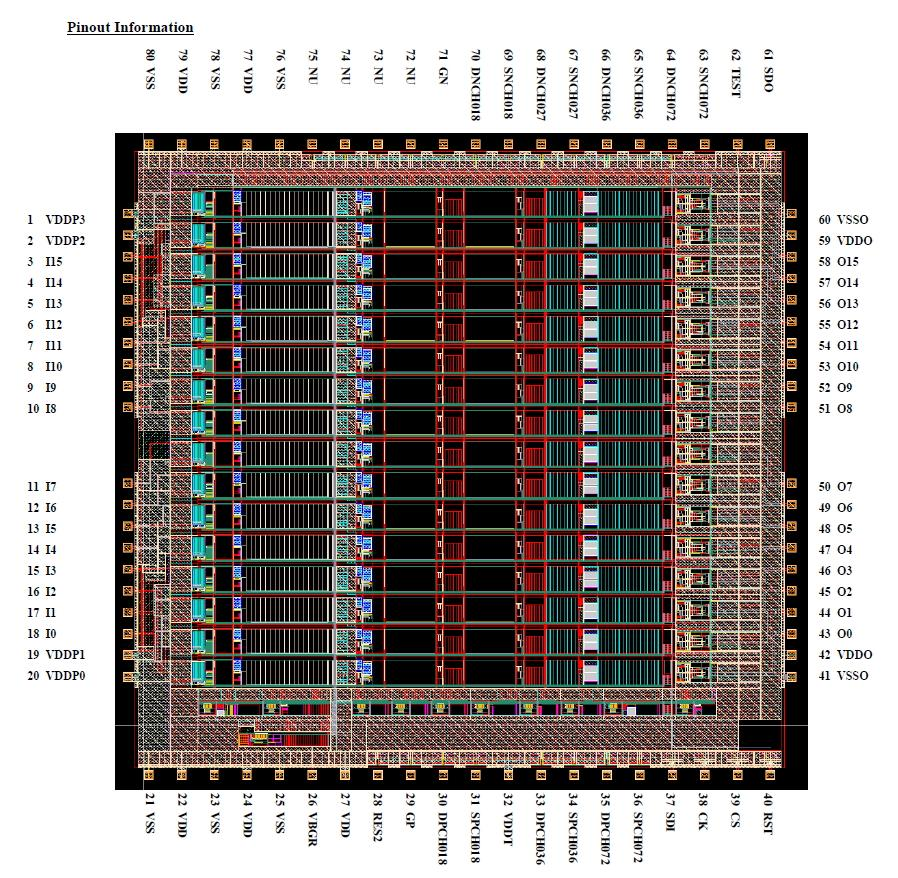
\includegraphics[width=\linewidth]{tpcce_FE_ASIC_pinout.jpg}
\end{cdrfigure}

This ASIC has now been through six design/fabrication/testing revision cycles; the latest data sheet is DUNE-doc-1484.
Prototypes from each cycle have been evaluated and characterized at room (300~K) and liquid nitrogen (77~K) temperatures.
During these tests the circuits have been cycled multiple times
between the two temperatures and operated without any change in performance.
Figure~\ref{fig:tpcce_shaper_out} shows the measured pulse response, along with
details on the adjustability of the gain, peaking time and baseline,
and the outputs of the BGR and temperature sensor.
These results are in close agreement with the simulations and indicate
that both the analog and the digital circuits and interface operate as
expected in a cryogenic environment.

\begin{cdrfigure}[Measured pulse response with details]{tpcce_shaper_out}{Measured pulse response with
 details on gain, peaking time and baseline adjustments}
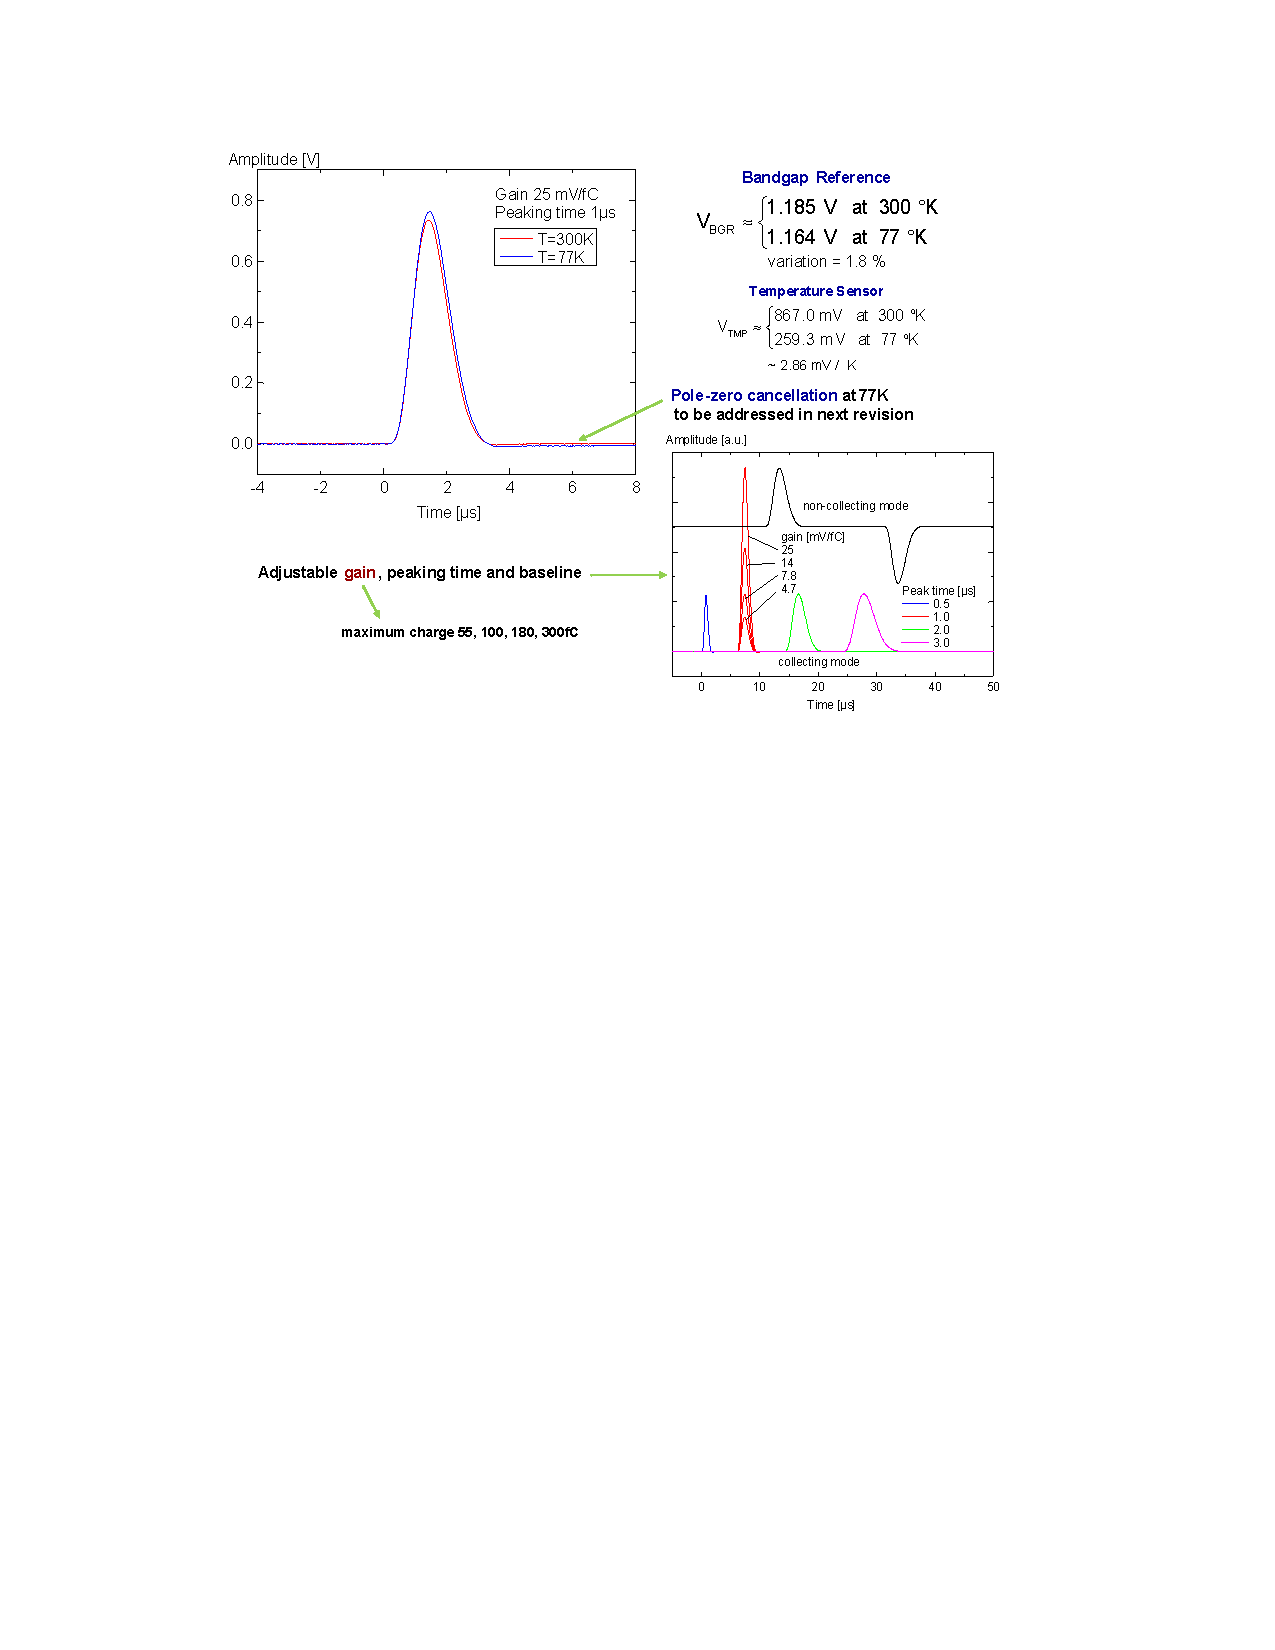
\includegraphics[width=\linewidth]{tpcce_shaper_out.pdf}
\end{cdrfigure}

\begin{cdrfigure}[Measured ENC vs filter time constant]{tpcce_enc}{
Measured ENC vs filter time constant from the latest prototype version of the FEMB
for two different gains, 14~mV/fC and 25~mV/fC. RT = room temperature and 
LN2 = liquid Nitrogen}
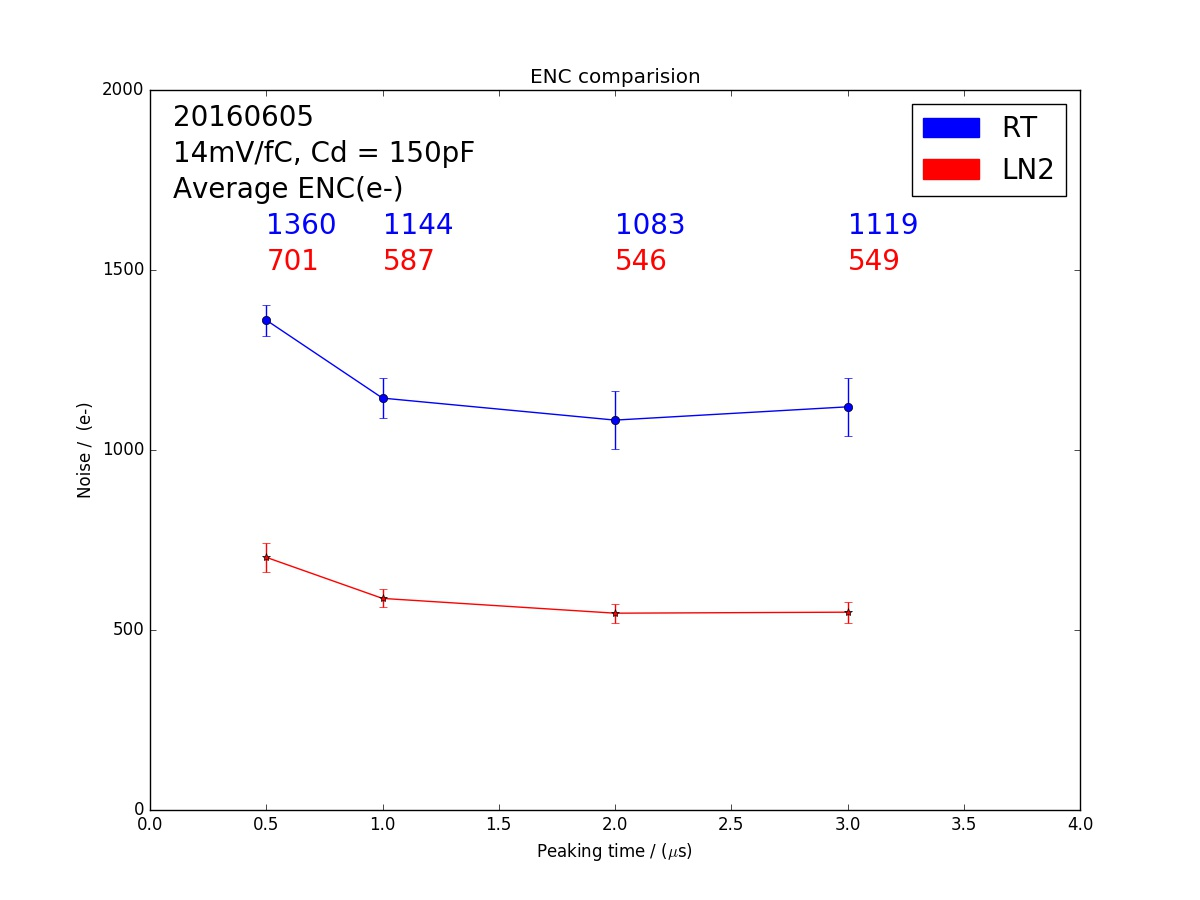
\includegraphics[width=4in]{tpcce_enc_14mV.jpg}
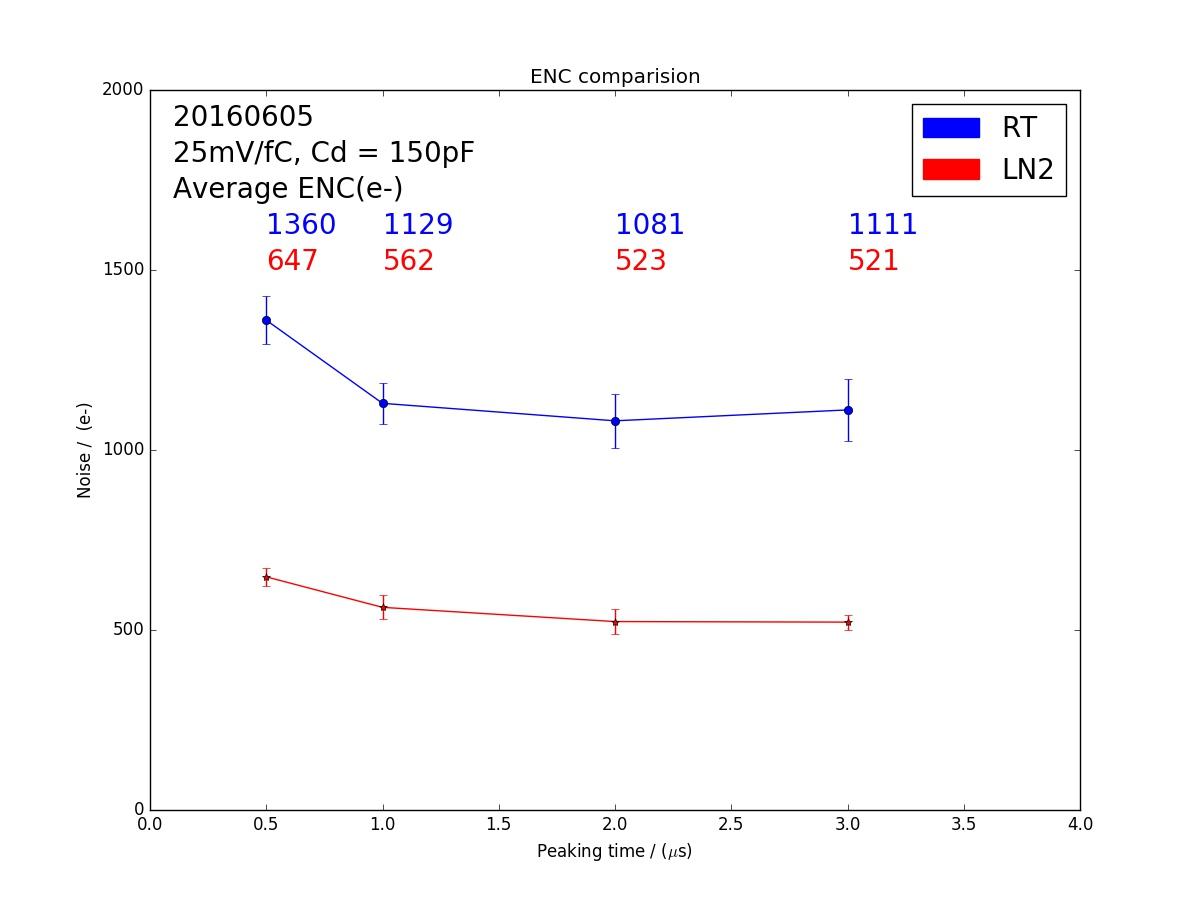
\includegraphics[width=4in]{tpcce_enc_25mV.jpg}
\end{cdrfigure}

Figure~\ref{fig:tpcce_enc} shows the measured Equivalent Noise Charge (ENC) versus 
filter-time constant (peaking time) for two different gains, where ENC is the value of charge 
(in electrons) injected across the detector capacitance that would produce at the output of the 
shaping amplifier a signal whose amplitude equals the output R.M.S. noise. These measurments
were made with prototype FEMBs at both room temperature (RT) and submerged in liquid
Nitrogen (LN2) with a wire-simulating input capacitance of $C_f~=~150$~pF.
In LN2, for peaking times $>$1~$\mu$s less than 600~e$^{-}$ was measured. For comparison,
a MIP travelling perpendicularly to the wire plane in the direction of wire spacing is
expected to deposit $\sim$~10,000~e$^{-}$ on the collection wires, for a worst-case
S:N$\sim$16:1.

Each channel is equipped with an injection capacitor which can be used
for test and calibration and can be enabled or disabled through a
dedicated register. The injection capacitance has been measured using 
a calibrated external capacitor. The measurements show
that the calibration capacitance is extremely stable, changing from
184~fF at room temperature to 183~fF at 77~K. This result and the measured
stability of the peaking time demonstrate the high stability of the
passive components with the temperature. Channel-to-channel and chip-to-chip
variation in the calibration capacitor are typically less than 1\%. Measurements are being carried
out on the individual test structures fabricated on this ASIC to
confirm device models and design guidelines.

The development of the ADC ASIC also uses the CMOS process (0.18~$\mu$m and 1.8V).
A 16-channel ASIC has been prototyped and tested.
The layout of the ADC ASIC is shown in Figure~\ref{fig:tpcce_ADC_ASIC}. 
The ADC ASIC has 12-bit resolution, options for 0.5, 1, and 2~MS/s sampling rate, a built-in FIFO, 
two 8:1 multiplexing and two pairs of serialized outputs.
The ADC is a complex design with 320,000 transistors, while the FE has 16,000.
The transistor design work has all been done following the rules for long cryo-lifetime.

\begin{cdrfigure}[The layout of the 16-channel ADC ASIC]{tpcce_ADC_ASIC}{The layout of the 16-channel ADC ASIC}
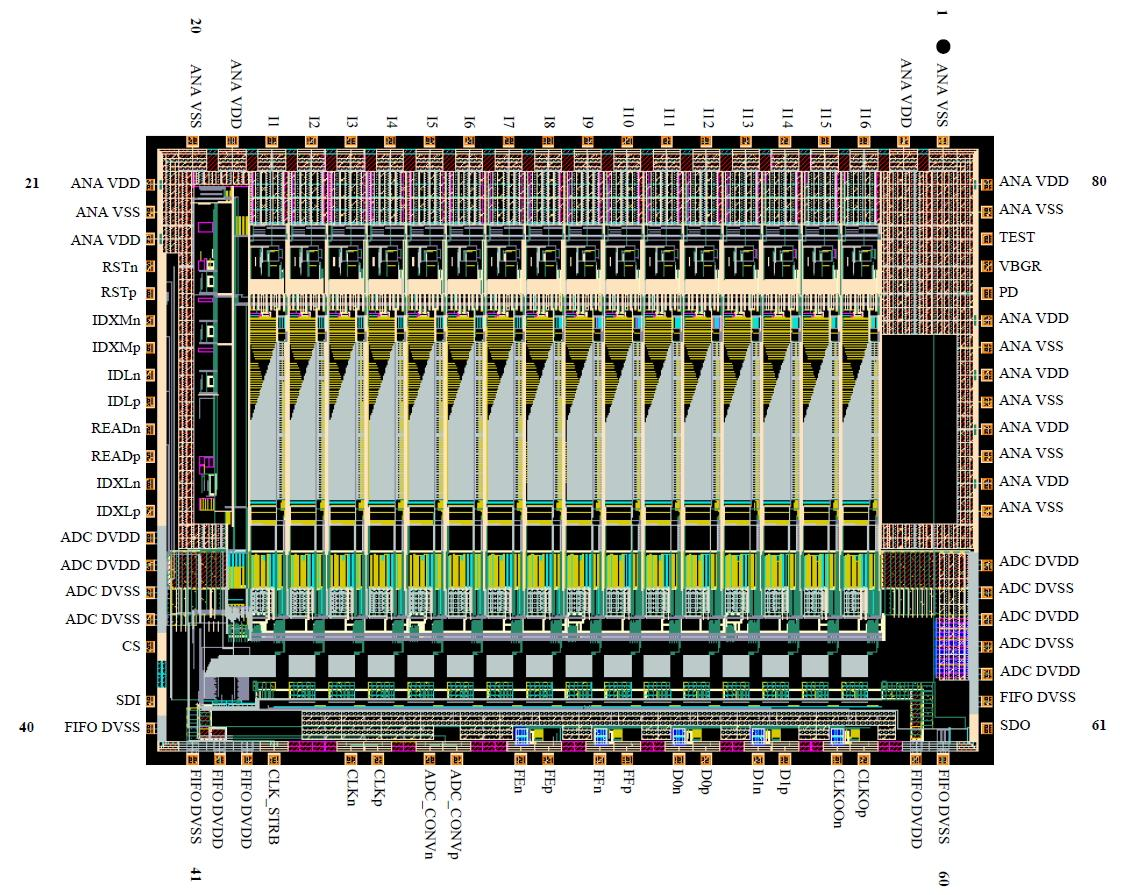
\includegraphics[width=\linewidth]{tpcce_ADC_ASIC_pinout.jpg} % New one
\end{cdrfigure}

The ADC ASIC has an input buffer with offset compensation to match the output of the FE ASIC.
The input buffer first samples the input signal (with a range of 0.2~V to 1.6~V),
then provides a current output after compensating for offset voltage error.
This current output is then supplied to the ADC which converts the input to digital in two phases.
The MSB (Most Significant Bit) 6~bits are first determined followed by the LSB (Least Significant Bit) 6~bits.
After the conversion the thermometer code is converted to binary and latched.
The output of ADC channel 16 can be monitored externally.
The data from the 16 ADCs are transferred in parallel to the FIFO block.
The built-in FIFO is 32~bits wide and 192~bits long,
and has full and empty indicator flags, needed to interface to an FPGA or digital ASIC.
The ADC along with the input buffers are biased internally using a bias generator and a bandgap voltage reference.
The bandgap voltage (VBGR) can be monitored and/or controlled externally.
It can be put in the low-power sleep mode, and woken up in less than 1~$\mu$s.

The ADC ASIC has now been through seven design/fabrication/testing revision cycles, 
the latest data sheet is DUNE-doc-1485.
Prototypes from each cycle have been evaluated and characterized at room (300~K) and liquid nitrogen (77~K) temperatures.
During these tests the circuits have been cycled multiple times.
The effective resolution with reference to the input referred noise is $\sim$11.6~bits at both 300~K and 77~K.
The differential non-linearity (DNL) is less than 4 LSBs for 99\% of ADC bins at both 300~K and 77~K.
The performance of the ADC meets the far detector requirements.

An analog front-end ASIC was adopted by the MicroBooNE experiment in 2010.\cite{noise_filter}
The fabrication and installation was successfully completed in early 2014, and now 
a total of 8,256 channels (516 FE ASICs in the LAr) instrument the MicroBooNE TPC. 
A total of 2,048 channels (128 FE ASICs and 128 ADC ASICs on 16 FEMBs in the LAr) instrument the 35-ton 
TPC, which has completed its data-taking.



%%%%%%%%%%%%%%%%%%%%%%%%%%%%%%%%
\subsubsection{Faraday box and interface to APA}
\label{subsubsec:ce_faraday_box}

Each FEMB will be enclosed in a Faraday box to provide shielding from noise, and to mount the FEMB 
to the APA. The current concept for Faraday box mounting is shown in Figure~\ref{fig:tpcce_box}. This
design is still being optimized for the ProtoDUNE detector.

\begin{cdrfigure}[Faraday box for the FEMB]{tpcce_box}{Faraday box for the FEMB.}
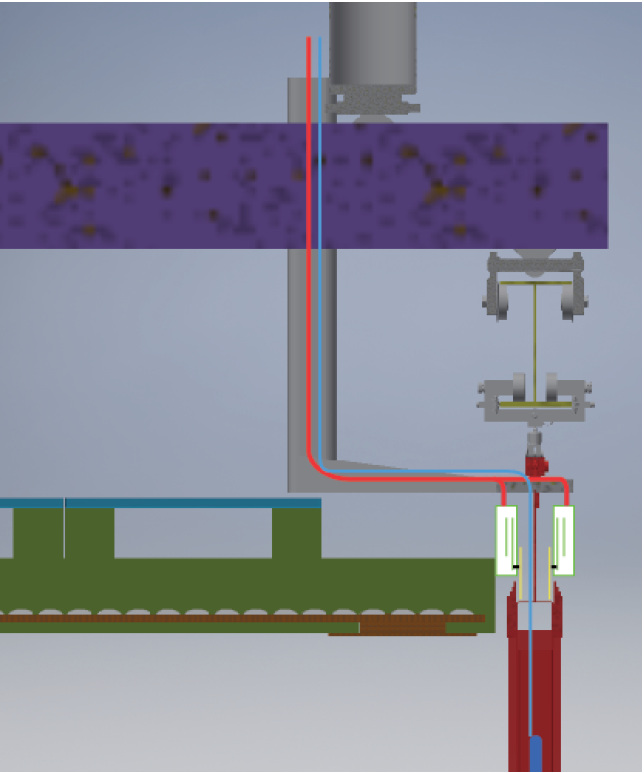
\includegraphics[width=3in]{tpcce_box_1.pdf}
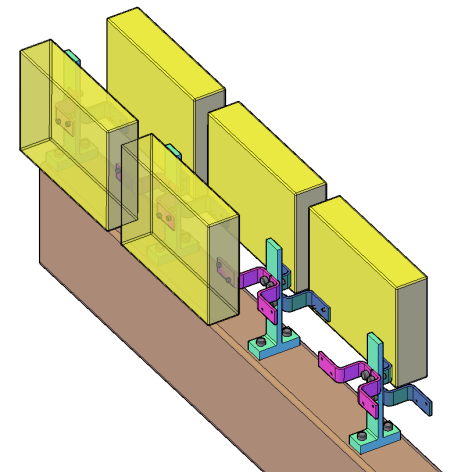
\includegraphics[width=3in]{tpcce_box_2.pdf}
\end{cdrfigure}

In addition to noise shielding, the Faraday box is designed to make the electrical connection 
between the FEMB and the APA frame, as defined in Section~\ref{subsec:ele_design}. Mounting 
hardware inside the Faraday box will connect the common plane of the FEMB to the box casing. The
box casing will be electrically connected to the APA frame via twisted conducting wire (not 
shown in Figure~\ref{fig:tpcce_box}). This is the only point of contact between the FEMB and
APA, except for the FE input amplifiers connected to the CR board, which also terminates to
ground at the APA frame, as shown in Figure~\ref{fig:tpcce_cr_board}.

In the DUNE far detector, the Faraday box will also route bubbles generated from the heat dissipated 
by the FEMBs away from the APA face for the APAs that have their FEMB installed on the bottom of
the APA. However, ProtoDUNE is only instrumenting FEMBs along the top of its APAs, so this feature
is not required.

%
%%%%%%%%%%%%%%%%%%%%%%%%%%%%%%%%
\subsection{Signal feedthroughs and cold cable}
\label{subsec:ce_feedthrough}

All LV and data cables inside the cryostat connect to the warm outside via flange PCB boards installed in feedthroughs
which are distributed along the cryostat roof (Fig.~\ref{fig:tpcce_FT_InternalCableRoute}).
The TPC data rate per APA, using the full event-buffer scheme described earlier,
is sufficiently low that it is within the capability of a single LVDS channel on copper,
with an overall 32:1 Mux and 80 $\sim$1~Gbps LVDS data channels per APA.
There is, therefore, no need for high-speed optical links inside the 
cryostat, so all cables inside the cryostat will be copper.
This has the significant benefit of avoiding a major R\&D effort which would be required to demonstrate
both functionality and adequate lifetime of optical converters in LAr.
In addition to the high-speed data-output channels,
LVDS connections will be made to each APA to distribute a clock signal and control information.
These data can be transmitted at a lower bit rate.
Optical fiber will be employed externally from the CE flange to the DAQ systems and slow control.

\begin{cdrfigure}[Conceptual design of signal/power feedthrough]{tpcce_FT_InternalCableRoute}{
The feedthrough configuration and internal cable routing. The left panel shows a cutaway view of the cryostat.
The right panel shows more detail at the Faraday boxes.}
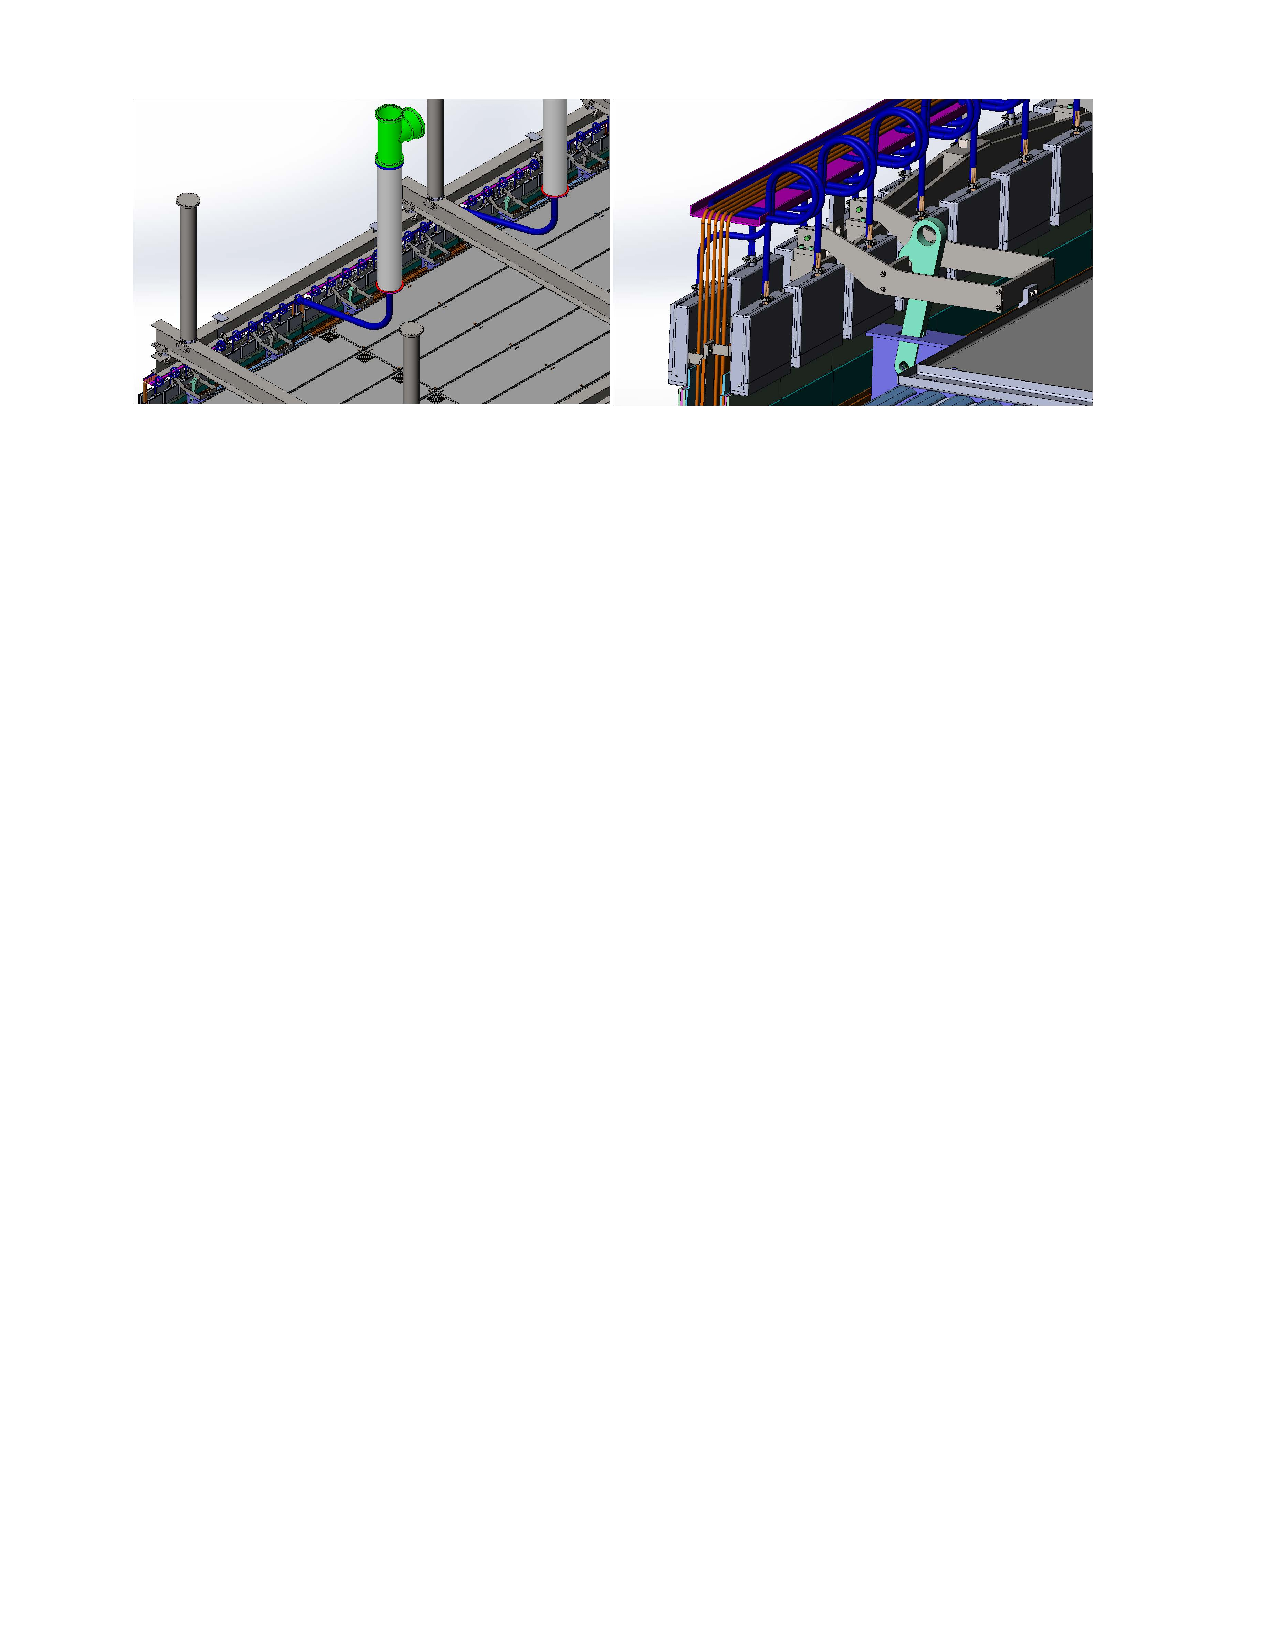
\includegraphics[width=7in]{tpcce_FT_InternalCableRoute.pdf}
\end{cdrfigure}

%
%%%%%%%%%%%%%%%%
\subsubsection{Signal feedthroughs}
\label{subsubsec:ce_feedthroughs}

\begin{cdrfigure}[Conceptual design of signal/power feedthrough]{tpcce_signal_FT}{
TPC signal/power feedthrough. The WIBs are seen edge-on in the left panel,
and in an oblique side-view in the right panel, which also shows the warm crate in a cutaway view.}
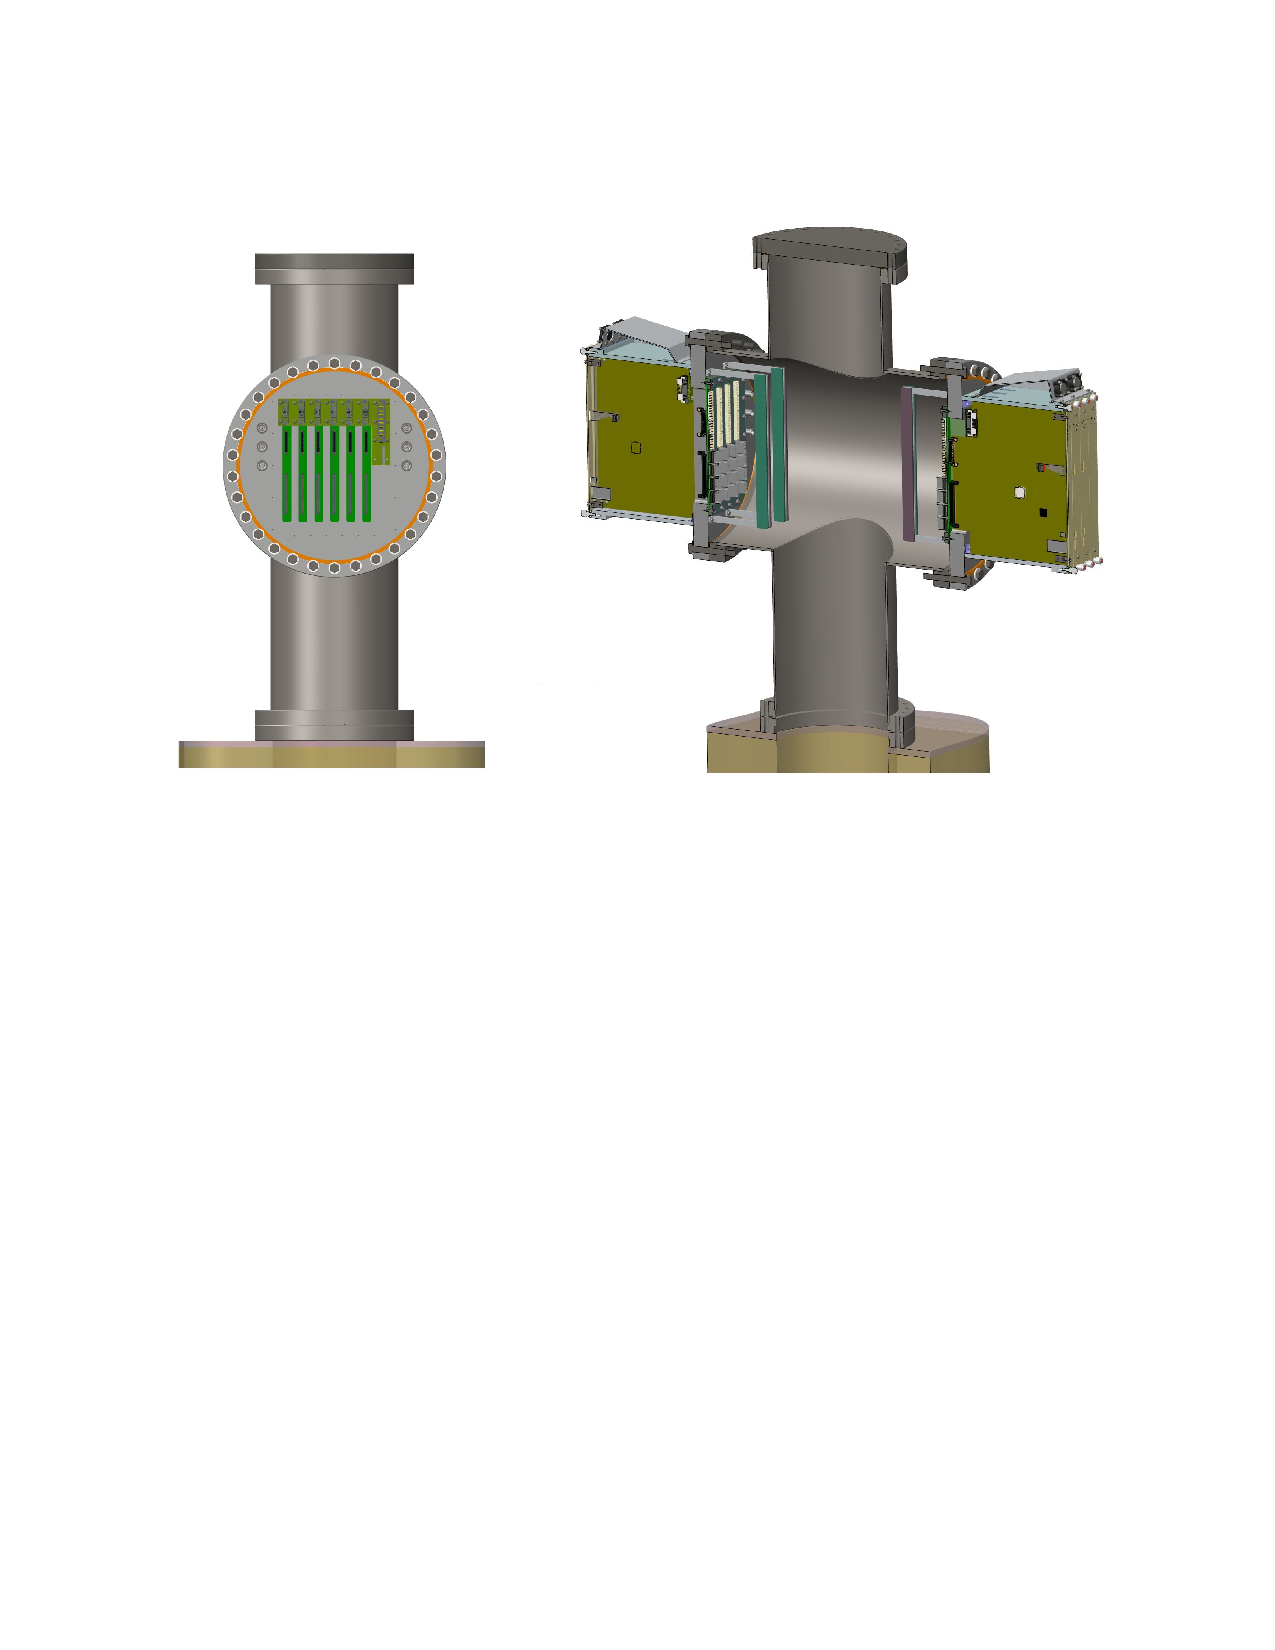
\includegraphics[width=7in]{tpcce_signal_FT.pdf}
\end{cdrfigure}

The ProtoDUNE feedthroughs are being developed in tandem with the SBND experiment because of their very similar needs.
The current ProtoDUNE design of the signal feedthrough includes a T-shaped pipe, CE flange, and warm electronics crate, as shown in Fig.~\ref{fig:tpcce_signal_FT}.
The wire-bias voltage cables will connect to standard SHV connectors machined directly into the flange,
so there will be no electrical connection between the LV and data connectors and bias voltage.
The other ends of the data and LV cables will be connected to the matching connectors on the FEMBs in the cryostat.
Based on a standard 14-in conflat flange,
each of these feedthroughs will serve the bias/power/digital IO needs of one APA, as shown 
in Figure~\ref{fig:tpcce_cable_routing}.  

\begin{cdrfigure}[TPC cable routing scheme]{tpcce_cable_routing}{TPC cable routing scheme for three APA section.}
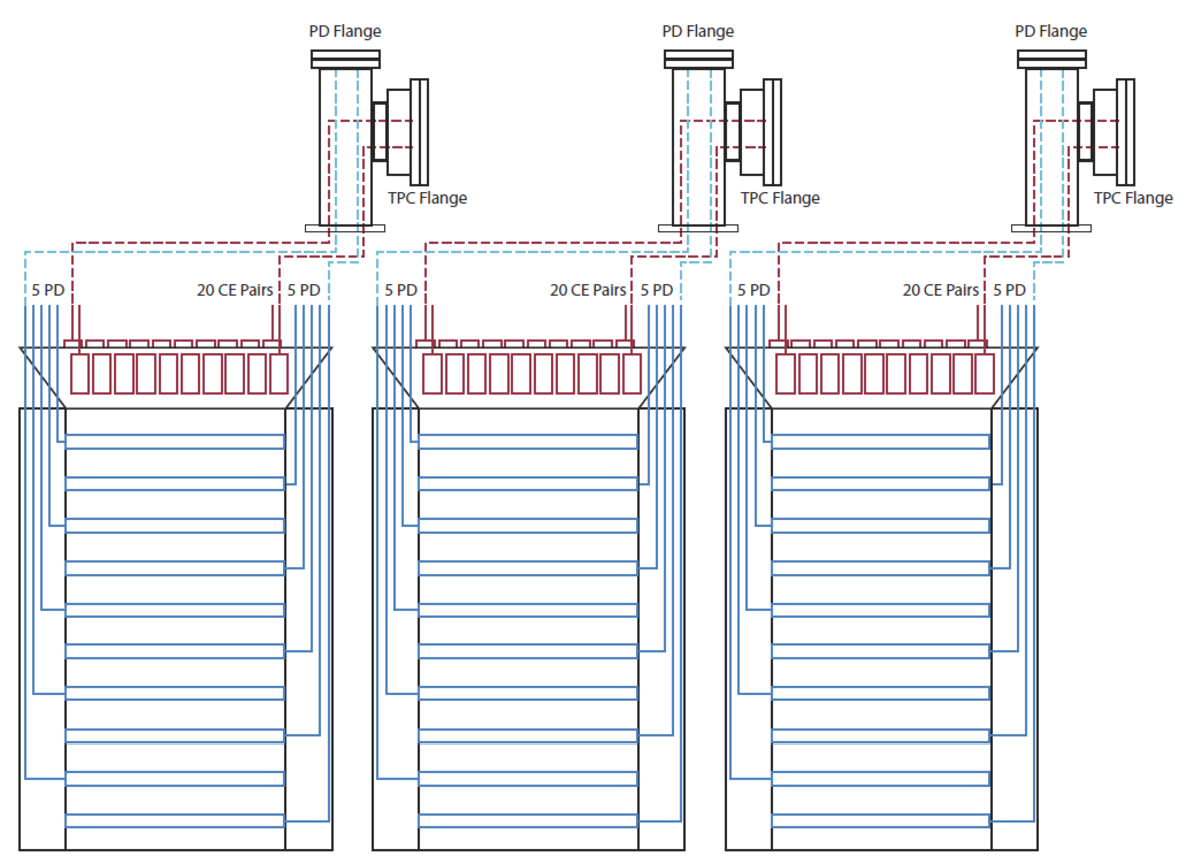
\includegraphics[width=0.9\linewidth]{tpcce_cable_routing.pdf}
\end{cdrfigure}

% All data, control, bias and power supply lines will be duplicated to
% provide redundancy to avoid the loss on an entire APA.
% Two APAs will be cabled to one feedthrough in ``chimneys'' in the roof of the cryostat that
% contain the support rods for the TPC planes.

For the protoDUNE detector APA there will be 20 electronics boards.
While the electrical connection requirements are straightforward,
the reliable gas tightness of the flange with an embedded circuit board has been fully verified.
The program for reducing contamination from the cable plant in the ullage
(the warmer gas phase at the top of the cryostat) 
is being carefully followed.
Measurements in the Materials Test Stand at Fermilab (described in Section 7.2 of the LBNE Closeout document).
have shown that impurities (principally O$_2$ and H$_2$O) embedded in objects submerged in the liquid argon do not result
in a decrease in electron-drift lifetime, whereas impurities in objects located in the ullage do, thus
the importance of minimizing the amount of material in the ullage.

%
%%%%%%%%%%%%%%%%  
\subsubsection{Data/control cable bundles}
\label{subsubsec:ce_data_cable}

\fixme{Gina says to simplify section and get rid of figures; still to do}

Data/control cable bundles will be used to send system clock and control signals in the LAr from the 
CE flange to the FEMB, stream the $\sim$1~Gbps high-speed data from the FEMB to the CE flange, and 
provide backup JTAG programming to the cold FPGA, in case the power-up programming fails to 
load from the onboard EEPROM. As described in Section~\ref{subsec:ce_intro}, each FEMB will 
connect to a CE flange via one data cable bundle, for 20 bundles between one APA and one flange.
Each data bundle will contain 12 low-skew Copper twin-axial cables with a drain wire, 
to transmit the following differential signals:

\begin{itemize}
    \item 4$\times$1.2~Gbps high-speed data
    \item One 50~MHz system clock
    \item One 2~MHz CONVERT clock
    \item 2 I2C control and configure (3 for COLDATA)
    \item 4 single-ended JTAG programming for the FPGA (not used for COLDATA)
\end{itemize}

Note that when the cold FPGA is replaced with the COLDATA ASIC, there
is a small change in signal assignments required, with one pair of
JTAG signals reassigned to the ``I2C-Like'' COLDATA slow control
interface, which uses three LVDS pairs, so that COLDATA will only
require 9 differential signals.

\begin{cdrfigure}[Samtec LV and data cable]{tpcce_samtec_cable}{Samtec data (left) and LV power (right) cable.}
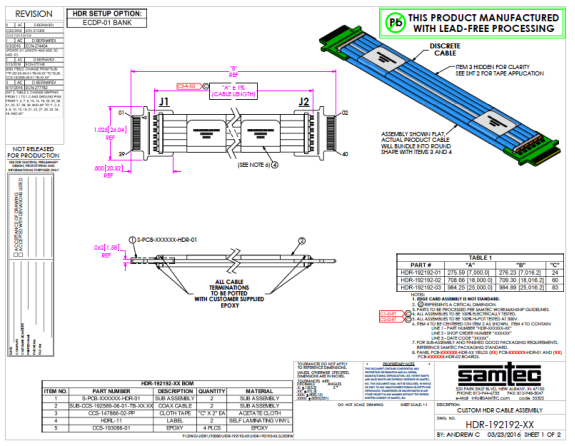
\includegraphics[width=5in]{tpcce_samtec_data.pdf}
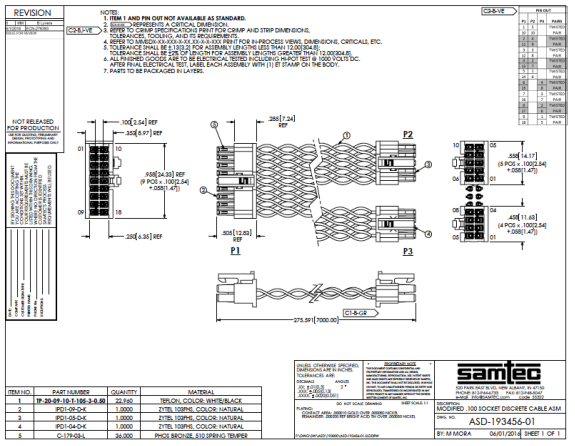
\includegraphics[width=5in]{tpcce_samtec_lv.pdf}
\end{cdrfigure}

ProtoDUNE will use Samtec 26~AWG twin-axial cable bundles with Samtec HSEC08 connectors to both
the FEMB mezzanine board and the CE flange, shown in Figure~\ref{fig:tpcce_samtec_cable}. The HSEC08
connectors lock into place with tabs on each side of the connector. A sample of the Samtec cable with
THV outer jacket has passed the LAr Materials Test Stand at Fermilab.

The Samtec 26~AWG cable has been
tested and demonstrated to have low enough dispersion that both the LVDS 50~MHz system clock and
$\sim$1~Gbps high-speed data can be recovered over 25~meters of room temperature (RT) cable, making this
a candidate cable choice for the DUNE far detector. However, for ProtoDUNE only the top APA
layer will be installed, so the cable length between the FEMB and CE flange will be approximately 7~meters.

\begin{cdrfigure}[Results from cable validation testing]{tpcce_samtec_results}{Eye diagrams 
from cable validation testing. {\bf Top Left:} 50~MHz system clock over 25~m room temperature 
(RT) Samtec 26AWG cable. For comparison, {\bf Bottom Left} shows the same clock over 
the heavier, prohibitively expensive Gore 24AWG cable. {\bf Top Right:} 1~Gbps data over 
7~m (ProtoDUNE length) RT Samtec 26AWG cable without active recovery by equalizers. {\bf Bottom Right} 1~Gbps
data over 25~m (DUNE length) RT Samtec 26AWG cable with active recovery.}
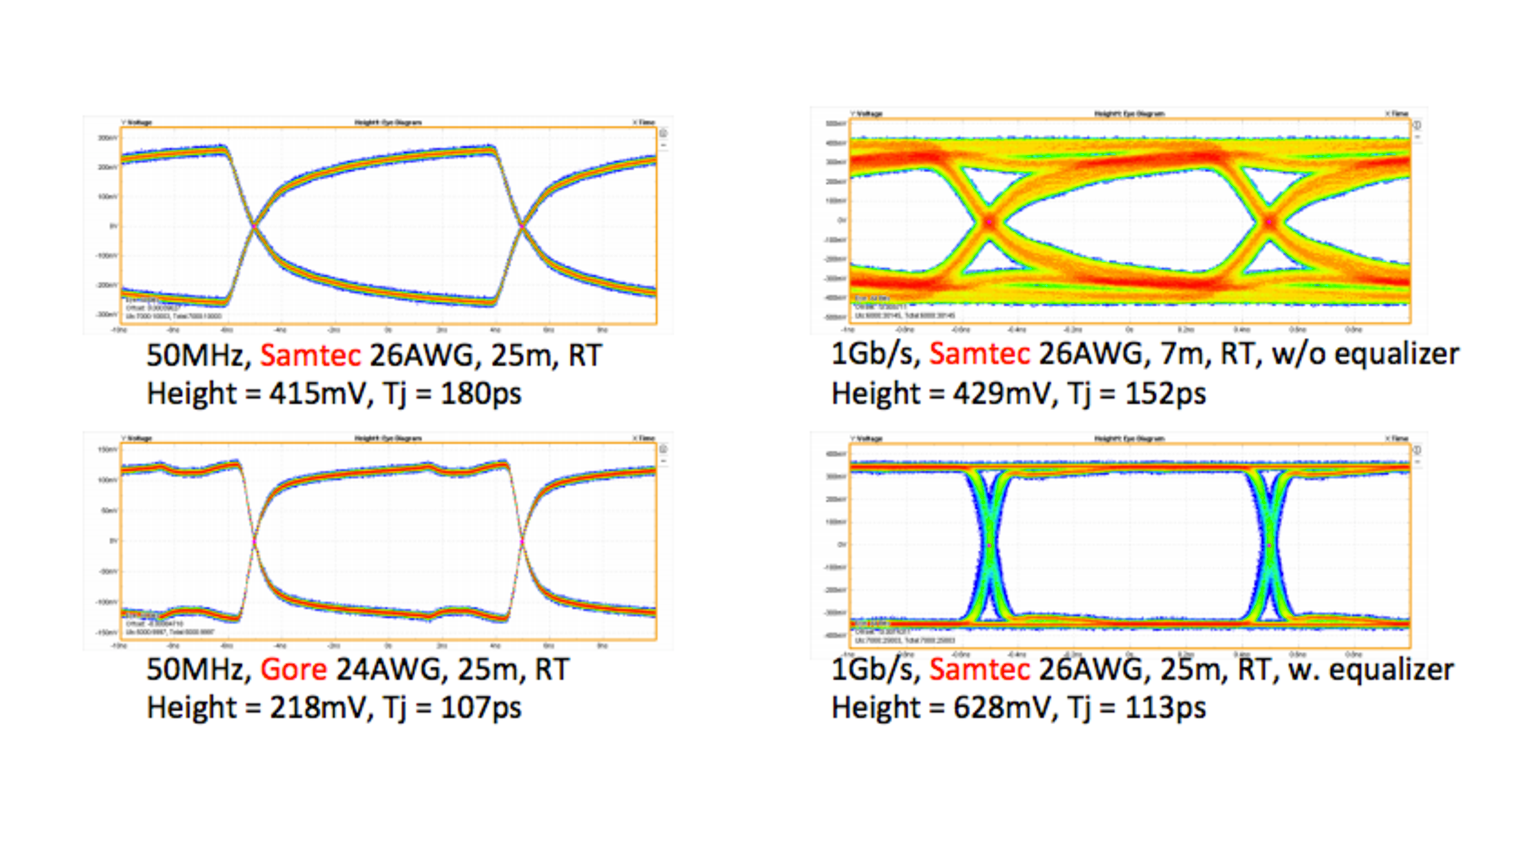
\includegraphics[width=1.0\linewidth]{tpcce_samtec_results.pdf}
\end{cdrfigure}

Figure~\ref{fig:tpcce_samtec_results} shows preliminary results from the DUNE cable 
validation testing. The eye diagrams show the edges of the differential signals after 
LVDS transmission over the specified cable types and lengths. The height of eye diagram shows the size 
of the recovered signal in mV and the slope of the rising and falling edges are jitter in picoseconds (ps). 
An eye diagram is sufficient to show that the edges of the differential signals can
be recovered, but not enough to demonstrate the bit error rate (BER).

The top left and bottom right eye diagrams in Figure~\ref{fig:tpcce_samtec_results} show 
that the Samtec 26~AWG cable allows recovery of both 50~MHz system clock and 1~Gbps digitized waveform 
data at RT over 25~m, the longest expected cable length in the DUNE far detector. 
The top right eye diagram shows that this cable also allows recovery at RT of the 1~Gbps data 
at the ProtoDUNE length of 7~m without active equalization. 
The Samtec 26~AWG cable has 
also passed a BER test, transmitting $10^{13}$ bits without error.

\subsubsection{LV Power Cable Bundles}
\label{subsubsec:ce_lvpower_cable}

The LV power will be provided in the LAr from the CE flange to the FEMB by bundles of 16 Samtec 
20~AWG twisted-pair wires, as shown in Figure~\ref{fig:tpcce_samtec_cable}. 1 IPD1 connector will
attach all 16 wires at the CE flange, and 2 IPD1 connectors will be attached to the FEMB (one to the
analog motherboard and one to the FPGA mezzanine. Like the data/control bundles, 20 LV wire bundles 
will bring power from one CE flange to one APA worth of FEMBs, and will be approximately 7~m long.

8 of the 16 wires will be power feeds, as described in Figure~\ref{fig:tpcce_lv_req}. The other 8 wires
will be attached to the common of the FE input amplifier, as described in Section~\ref{subsec:ele_design}. For
a single FEMB, the resistance is $<30$~mOhm at RT or $<10$~mOhm at LAr temperature. For
all 20 FEMBs, each APA will have a copper cross-section of approximately $80~\mathrm{mm}^2$, with
a resistance $<1.5$~mOhm at RT or $<0.5$~mOhm at LAr temperature.

\begin{cdrfigure}[LV power feed wire specifications]{tpcce_lv_req}{Samtec LV power feed wire 
specifications.}
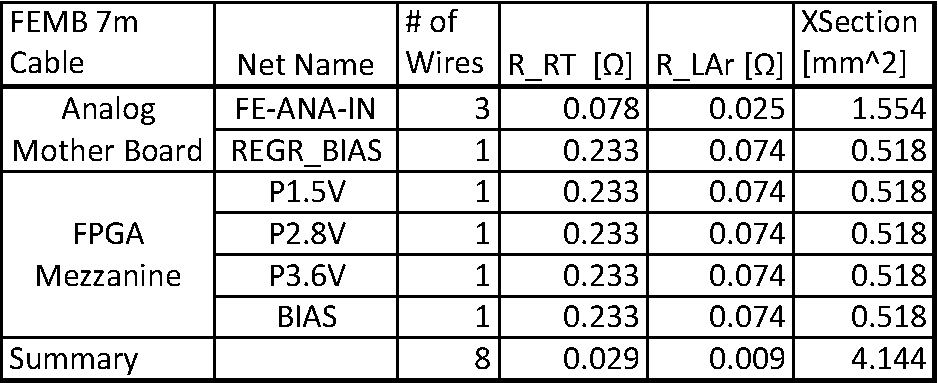
\includegraphics[width=4in]{tpcce_lv_req.pdf}
\end{cdrfigure}

\subsubsection{Wire Bias Cables}
\label{subsubsec:ce_bias_cable}

The wire-bias cables must deliver voltages up to two or three thousand Volts with less than a 
couple of milliAmps.

The bias voltages are applied to the X, V, and G wire layers, three field cage terminations, 
and an electron diverter, as shown in Figure~\ref{fig:tpcce_cr_board}. The voltages are supplied 
through eight SHV connectors mounted on the CE flange. RG-316 coaxial cables carry the voltages 
from the CE flange to a patch panel PCB which includes noise filtering mounted on the top 
end of the APA. From there, bias voltages are carried by single wires to 
various points on the APA frame.

Field cage noise filters and termination are also located on a small PCB mounted on or near 
the patch panel. Bias voltage filters are also mounted on or near the electron diverter.

It will be important that all cables and connectors be somewhat rugged,
locking and able to withstand a minimum of several tens of mating cycles.
Unfortunately, because of size and space limitations, the type of connectors we need are not keyed,
so a labeling scheme and caution when connecting cables are the only options available.

\subsection{Warm Interface Electronics}
\label{subsec:warm_interface_elec}

The ProtoDUNE warm interface electronics are housed in a small crate
attached directly to the cryostat flange.  The crate contains one
Power and Timing Card (PTC), up to five Warm Interface Boards (WIBs) and a passive
backplane which fans out signals and LV power from the PTC to the WIBs.

\begin{cdrfigure}[Conceptual design of CE flange]{tpcce_ceflange_sbnd}{Exploded view of 
the CE flange for SBND (ProtoDUNE has 5 WIBs).}
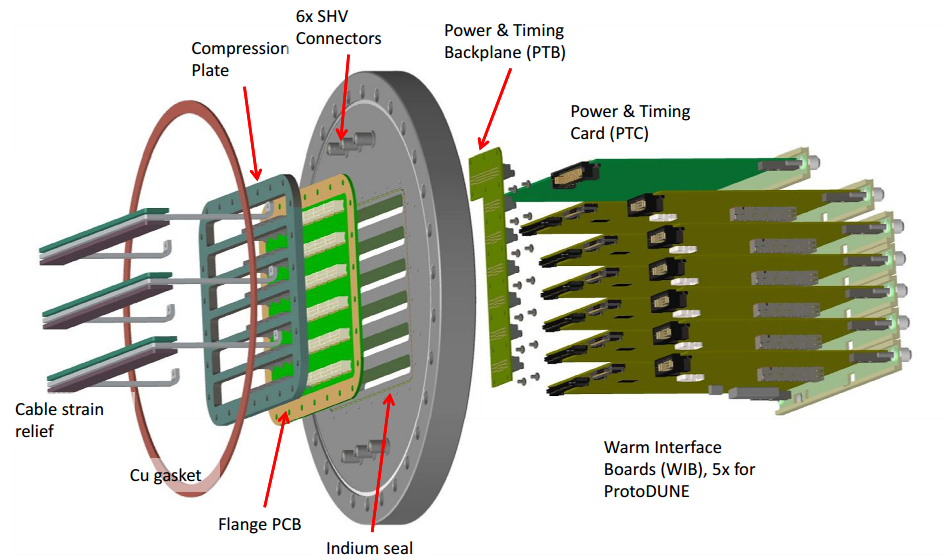
\includegraphics[width=0.9\linewidth]{tpcce_ceflange_sbnd.png}
\end{cdrfigure}

The WIB is the interface between the
DAQ system (based on either the RCE or FELIX) and up to four
FEMBs. It receives the system clock timing and control signals from the
timing system and provides processing and fan-out to the four
FEMBs. The WIB also receives the high-speed data from the four 
FEMBs and transmits it to the DAQ system over optical
fiber.  Figure~\ref{fig:tpcce_ceflange_sbnd} shows the TPC warm electronics
flange (SBND design). The WIBs are attached directly to the TPC
readout electronics flange on the cryostat feedthrough. The flange
board is a PCB with connectors to the cold signal and LV cables fitted
between the compression plate on the cryostat side, and sockets for
the WIB on the warm side. Cable strain relief is also provided
directly on the flange, which is mounted vertically to the cryostat
feedthrough.

\subsubsection{Power and Timing Card}
\label{subsubsec:power_timing_card}

\begin{cdrfigure}[PTC and timing]{tpcce_wib_timing}{Power and Timing Card (PTC) 
and timing distribution to the WIB and FEMBs.}
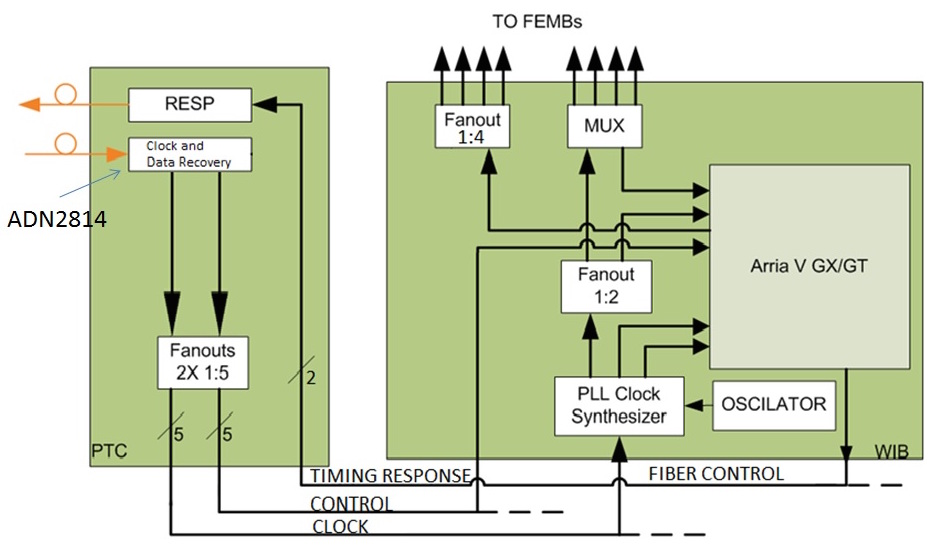
\includegraphics[width=0.9\linewidth]{tpcce_wib_timing.jpg}
\end{cdrfigure}

In addition to the WIB, the warm interface electronics contains a
Power and Timing Card and a Power and Timing Backplane
(PTB). The PTC provides a bidirectional fiber interface to the
ProtoDUNE clock system.  The received data is separated into clock and
data using a clock/data separator.  The clock and data
streams are separately fanned-out to five WIB via the power/timing
backplane. Details are shown in
Figure~\ref{fig:tpcce_wib_timing}. The PTC fans the clocks out to the WIB over the
PTB, which is a passive backplane attached directly to the PTC and
WIBs, shown in Figures~\ref{fig:tpcce_ceflange_sbnd} and~\ref{fig:tpcce_dune_ptb}.

\begin{cdrfigure}[WIB and LV power]{tpcce_wib_power}{LV power distribution 
to the WIB and FEMBs. 200W is for a fully-loaded crate 
with the majority of the power dissipated by the 20 cold FEMBs in the LAr.}
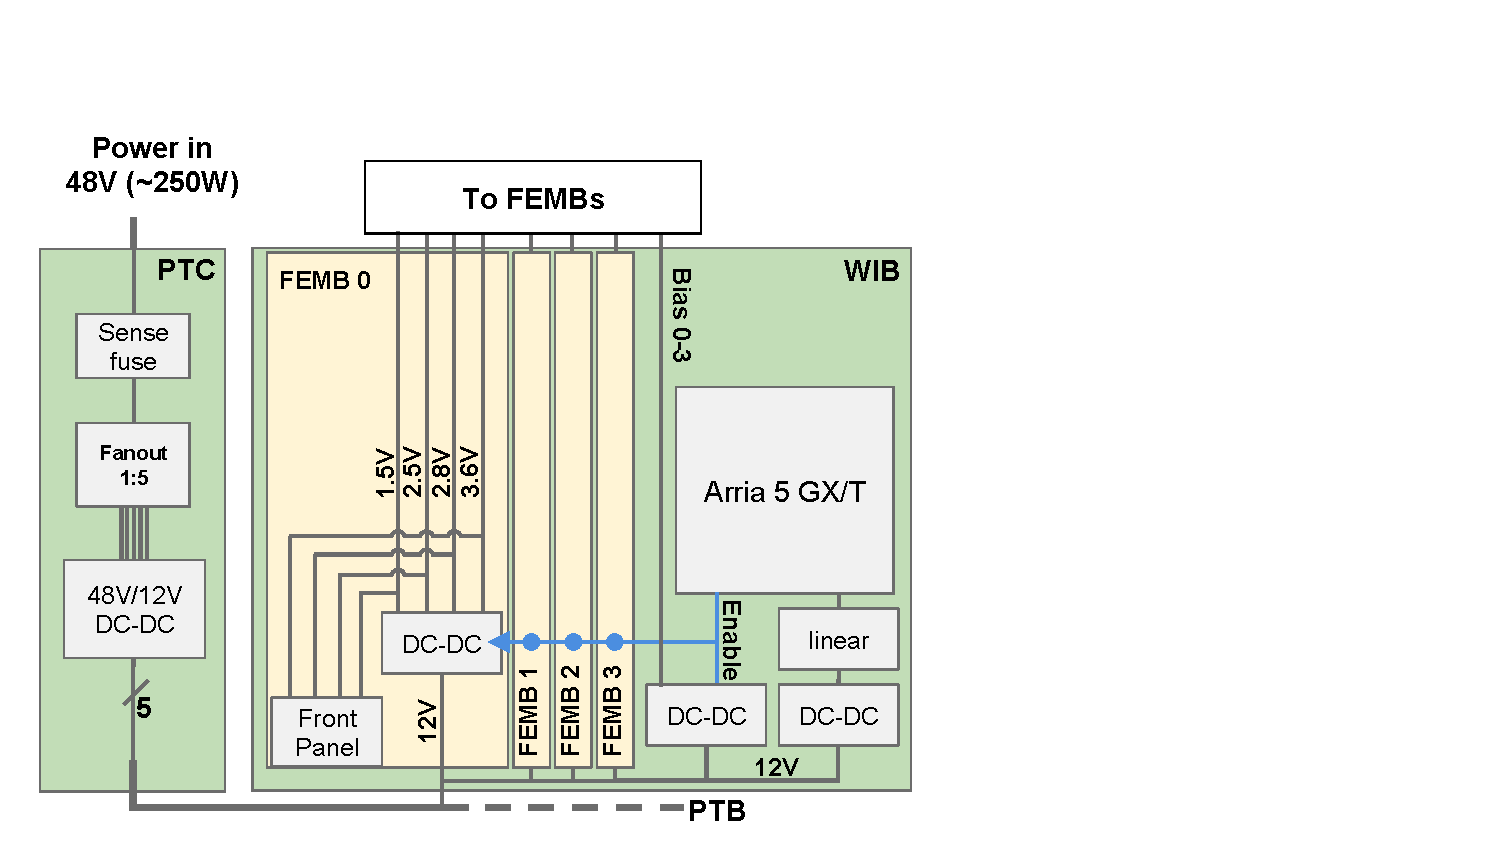
\includegraphics[width=0.7\linewidth]{tpcce_wib_power.pdf}
\end{cdrfigure}

The PTC also receives the low voltage power for the entire cold
electronics connected to that flange, approximately 200W at 12V for a
fully-loaded flange (5~WIB + 20~FEMB). The LV power is then fanned out
on the PTB to each WIB, which provides the DC/DC conversion and fans
the LV power out to each of the cold FEMBs supplied by that WIB, 
as shown in Figure~\ref{fig:tpcce_wib_power}. The 
majority of the 200W drawn by a full flange is dissipated in the LAr
by the cold FEMB.

ProtoDUNE has 6 cryostat signal feedthroughs with warm interface electronics. 
If the system clock is received by the PTC, it will require 6 dual fiber links.

\subsubsection{Warm Interface Board}
\label{subsubsec:warm_interface_board}

The WIB receives the separated clock and data from the timing system from the backplane
as shown in Figure~\ref{fig:tpcce_dune_wib}. Each WIB in ProtoDUNE will contain a 
unique IP address for its UDP slow control interface. The IP address for the WIB is 
derived from a crate and slot address: the crate address is generated on the PTC 
board via dipswitches and the slot address is generated by the PTB slot, numbered 
from one to five, shown in Figure~\ref{fig:tpcce_dune_ptb}. Note that the WIB also has 
connectors to receive LV power on its front panel, bypassing the PTC.

The WIB is also capable of
receiving the encoded system clock over bi-directional optical
fibers on the front panel; in this scenario, the warm electronics would require 
30 fiber links to the clock system. The clock will be divided by two using either
the FPGA or an on-board clock synthesizer chip to provide the 50~MHz
clock required by the cold electronics.  The clean clock and processed
control stream is fanned out to up to four FEMBs.

\begin{cdrfigure}[Warm Interface Board]{tpcce_dune_wib}{Warm interface board (WIB). Note 
that front panel inputs will include a LEMO connector and alternate inputs for LV power.}
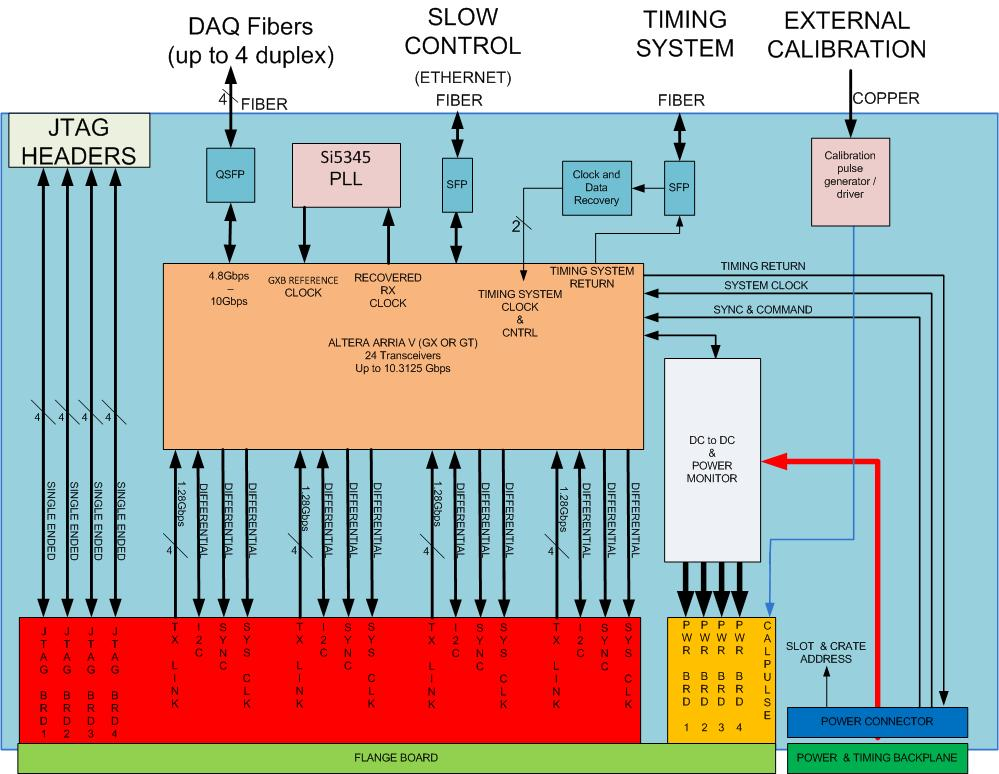
\includegraphics[width=0.9\linewidth]{tpcce_dune_wib.jpg}
\end{cdrfigure}

The FPGA on the WIB is an Altera Arria V GT variant, which requires a
125~MHz clock for its state machine which is provided by crystal
oscillators onboard the WIB. The GT variant of the Arria V
transceivers can drive the high-speed data to the DAQ up to
10.3125~Gbps per link, which is capable of transmitting all data from
two FEMB (2$\times$5~Gbps) on each link. However, the current design is to
use a QSPF socket on the WIB, and deliver $\sim$5~Gbps on four optical fibers 
(1 fiber per FEMB) to two RCEs. The FPGA also has Gbps Ethernet
transceiver I/O, also using the 125~MHz clock, which provides
real-time digital data readout to slow control.

\begin{cdrfigure}[Power and timing backplane]{tpcce_dune_ptb}{Power and Timing Backplace (PTB).}
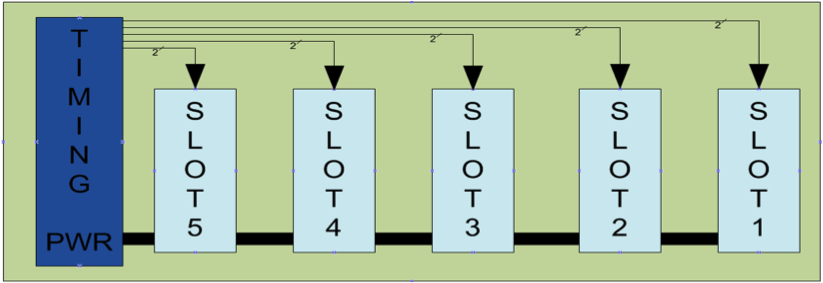
\includegraphics[width=0.7\linewidth]{tpcce_dune_ptb.png}
\end{cdrfigure}


%
%%%%%%%%%%%%%%%%
\subsection{External Power and Cables}
\label{subsec:ce_feedthrough_power}

The LV power to the FEMB and WIB will be supplied by Weiner MPOD power supplies. 
The power-per-channel for the FE electronics is designed be about 25~mW in the LAr.
Including power for the WIB, a fully loaded WIB (1 WIB plus 4 FEMBs) will require
12V and draw approximately 3.3~Amps. Therefore, a full WEC (5 WIBs + 20 FEMBs) will
require 12V and draw approximately 16~Amps, for a total power of almost 200~W, as 
described in Section~\ref{subsubsec:power_timing_card}.

Each MPOD LV unit has 2 DSUB37 connectors, each with 4 channels of LV output, including negative
and positive sense wires, as shown in Figure~\ref{fig:tpcce_mpod_top}. Each channel has 3 pins
of negative output and 3 pins of positive output. 5 of the 8 channels
will provide the 12V/3.3A to each WIB via the PTC, and 1 channel will provide LV power 
to the PTC itself, with 2 of the 8 channels unused.

\begin{cdrfigure}[MPOD DSUB37 top connector]{tpcce_mpod_top}{MPOD DSUB37 top connector.}
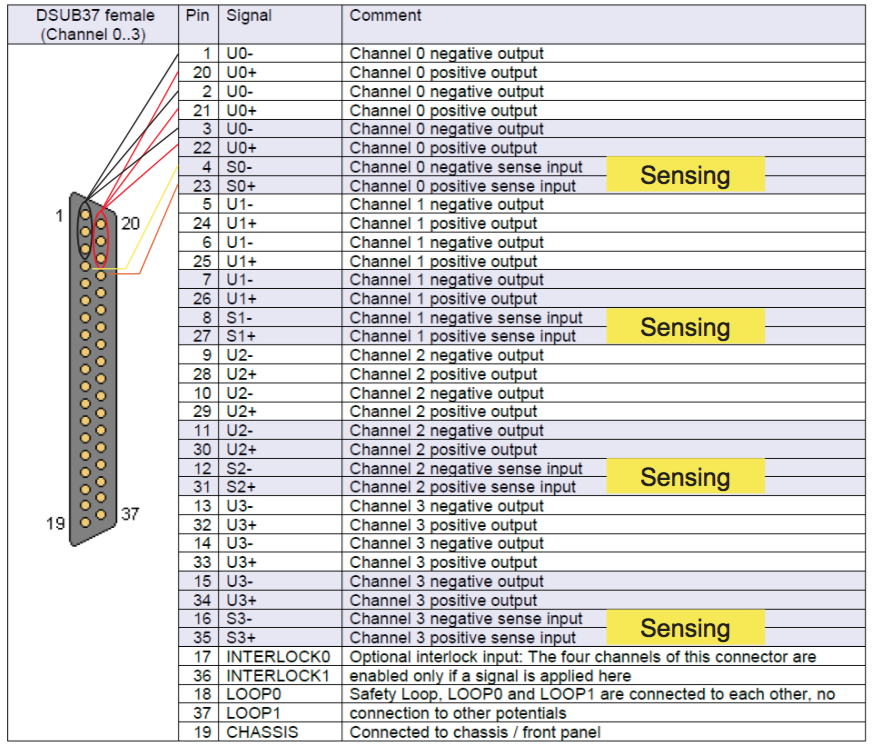
\includegraphics[width=1.0\linewidth]{tpcce_mpod_top.png}
\end{cdrfigure}

Each MPOD wire-bias voltage unit will supply the wire bias voltage to 8 SHV connectors 
at the CE flange. One MPOD chassis contains 3 LV and 3 wire-bias units, and will therefore 
supply all the low and wire bias power to three TPC APA cold electronics read-out units, 
requiring a total of 2 MPODs in the detector racks.

%
%%%%%%%%%%%%%%%%
\subsubsection{Low Voltage Cable}
\label{subsubsec:ce_feedthrough_lv}

The low voltage cable will be the fused DSUB37 connectors used by MicroBooNE to 
supply the power to the FE ASICs in that detector. The bottom of the fuse PCB at the MPOD 
end of the cable is shown in Figure~\ref{fig:tpcce_fused_cable}. Each of the 3 output pins on
each channel will be tied together in parallel 
going to one wire large enough to carry the full supply voltage. Fuses can optionally be 
populated on each output pin as shown in Figure~\ref{fig:tpcce_fused_cable}; however, if
fusing is not selected, the pins will be connected with 0~Ohm resistors. The fusing would be
the final protection: the main protection with be the Over Current protection
on the MPOD, which will be set above the 3.3A required by each WIB, but below the
combined fuse value.

\begin{cdrfigure}[Bottom of the fuse PCB]{tpcce_fused_cable}{Bottom of the fuse PCB at the MPOD end of the cable.}
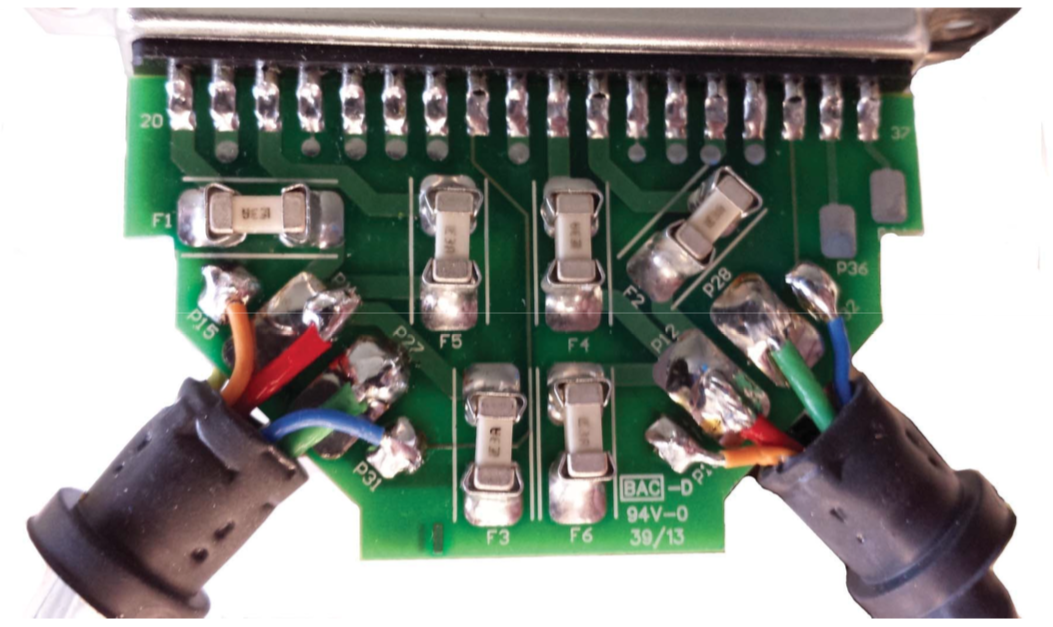
\includegraphics[width=0.7\linewidth]{tpcce_fused_cable.png}
\end{cdrfigure}

The 5 separate 12V/3.3A channels to the WIBs will be delivered to the WEC at the PTC described
in Section~\ref{subsubsec:power_timing_card}. The PTC will have two normal DSUB37 connectors to
attach the LV power cable. The fusing for the sense wires will be implemented on the PTC.

The PTC will fan the LV out to the WIB over the backplane. Each WIB will do the DC-to-DC conversion
from 12V to the voltages required by the FEMBs shown in Figure~\ref{fig:tpcce_lv_req} and 
distribute those voltages over the LV copper cable inside the cryostat to up to four FEMBs, as described in 
Section~\ref{subsubsec:warm_interface_board}.

%
%%%%%%%%%%%%%%%%
\subsubsection{Wire Bias Voltage Cable}
\label{subsubsec:ce_feedthrough_wirebias}

Each anode plane assembly requires three bias voltage connections 
at $+$820V, $-$370V, and $-$665V, as described in Section~\ref{subsec:ce_wire_bias}.
The current on each of these supplies is expected to be zero at normal operation.
However the ripple voltage on the supply must be carefully controlled 
to avoid noise injection into the front-end electronics.

RG-58 coaxial cables will connect the wire bias voltages from the MPOD to the standard SHV
connectors machined directly into the flange, so there will be no electrical connection between 
the LV and data connectors and bias voltage. The length of the cables from the Weiner MPODs
to the CE flanges is estimated to be 18~meters.

%
%%%%%%%%%%%%%%%%
\subsubsection{Optical Fiber}
\label{subsubsec:ce_optical_fiber}

Optical fiber will be the only connection out of the Faraday box provided by the WEC to either 
the DAQ or slow control. Each WIB will use QSFP sockets, so each WIB/RCE connection will require 
4 pairs of fiber, as described in Section~\ref{subsubsec:warm_interface_board}.  ProtoDUNE has 
30 WIB, so it will require 120 pairs of optical data fiber. MPO multimode fiber cable assemblies 
are being considered; however the final choice has not been made. The optical fibers from
the CE flanges to the DAQ room are an estimated 30-40m in length.

Duplex LC optical fiber is under consideration to transmit one GIG-E connection from each
WIB to slow control. The WIB will report each FEMB current draw to slow control, and the 
current draw for each WIB can be monitored by slow control at the MPOD.

